\chapter{Characterising physical abilities} % Main chapter title

\label{ch:phisical_ability_metrics} % Change X to a consecutive number; for referencing this chapter elsewhere, use \ref{ChapterX}


This chapter starts with an an overview of various physical ability metrics for humans and robots, aiming to provide an unifying view of their physical abilities and set the stage for their use in human-robot collaboration scenarios.

The primary focus is put on the polytope-based family of metrics, as one of the well known physical ability metrics for both robots and humans. These metrics enable a unified and accurate representation of their individual abilities. By expressing individual abilities in a unified polytope form, the common physical abilities in collaboration scenarios can be computed using polytope algebra operations, and represented in polytope form as well.

Numerous polytope-based physical ability metrics have been developed in the literature. Therefore, section \ref{ch:poly_metrics} presents a comprehensive overview of common polytope-based metrics applicable to both humans and robots. Additionally, section \ref{ch:collab_metrics} explores their application in calculating the joint physical abilities of humans and robots when engaged in physical interactions to accomplish specific tasks. Finally the section \ref{ch:collab_metrics_overview} concludes the chapter and provides a structured synthesis of common polytope formulations.

% \todos{rewrite + list the chapter sections at the end}.

% \todos{
% \begin{itemize}
%     \item This chapter brings the overview of different physical ability metrics for humans, robots and their collaboration
%     \item The chapter further concentrates on polytope based physical ability metrics
%     \item it brings the most common formulations of different polytope based metrics for humans and robots
%     \item it shows how these metrics can be used to characterise the joint abilities in case of physical human robot interaction
%     \item finally it brings a generic polytope algebra based view on different polytope base physical ability metrics and their categorisation with respect to their formulation
% \end{itemize}
% }

\section{Common physical ability metrics}
% \todos{
% \begin{itemize}
%     \item Physical ability metrics are defined as mapping of the actuation space limits of robots and humans to the cartesian / task space 
%     \item many different metrics in the literature
%     \end{itemize}
% }

Physical ability metrics describe how different properties of robotic systems, such as the actuator limits and kinematic structure, as well as different biomechanical and biological limitations of human bodies, influence their respective capacity to execute movements, generate forces, achieve different precision levels or generate other physical quantities necessary to execute a certain task.

They are important tools for the analysis and design of robotic manipulators\cite{patel2015manipulator} as well as for defining the tasks they are capable of executing \cite{Pholsiri2015task}. In case of humans, they are used to ensure human safety by studying the ergonomics of different tasks and workspaces \cite{Golabchi2015}. Finally, they have a great potential to be used in human-robot collaboration scenarios to characterise joint physical abilities of robots and humans, with the aim to improve the quality, performance and safety of their physical interaction.

%However, not all the physical ability metrics are made equal. 
Many different metrics, both for humans and robots, were developed in the literature having a varying degree of complexity and physical interpretation, as well as different scope and accuracy.
Therefore, this section brings an overview of different physical ability metrics for robots and humans and discusses their potential use for human-robot collaboration.

\subsection{Metrics in robotics}
In robotics, physical abilities are characterised as different performance indicators, establishing the relationship between the robot's actuator limits (joint positions, velocities, torques, etc.), its kinematics and dynamics equations, and the achievable sets of different task related physical values, such as achievable positions, velocities, external wrenches and similar. The metrics quantifying different physical abilities are usually divided in two groups with respect to their scope: \textit{Global} and \textit{Local} metrics  \cite{russo2022measuring}. 

Global metrics present robot state independent metrics evaluated by taking in consideration all the possible robot states.
One example of such metric is the robot's reachable workspace \cite{Gosselin1991Synthesis,Vahrenkamp2016,kucuk2005robot}, characterising the set of cartesian positions the robot can reach given its geometry and the limitations of its actuator's positions. More generally, workspace analysis based tools find the set of robot's reachable cartesian positions given the limitations of its actuators, its kinematics and dynamics and different task related variables. Examples of such metrics are  constant orientation workspace \cite{Merlet1999Determination} representing robot's reachable positions with a given fixed orientation, singularity free workspace \cite{Jiang2008} representing the reachable positions without no singular configurations, or wrench closure workspace \cite{gouttefarde2006determination,Lau2011} which corresponds to robot's reachable positions guaranteeing the ability to apply certain set of wrenches.
One traditional application for such performance metrics is robot dimensional design, as they enable verifying and guaranteeing that the robotic system, being designed, is compliant with all the requirements of the tasks. 
However, these reachable workspace analysis tools have relatively complex geometry which can be challenging to exploit when it comes practical applications. 

A different set of global metrics, often specified in manufacturer's data-sheets, are different scalar metrics representing the robot's physical abilities based on finding the \textit{worst-case} (minimal) or \textit{best-case} (maximal) values of different task related values within the workspace. These metrics guarantee certain physical ability values for a given robot, such as robot's payload, its \textit{worst-case} carrying capacity, robot's \textit{worst-case} positioning accuracy or positioning repeatability \cite{russo2022measuring}. 
Therefore, they are often used evaluate if a certain robotic system is suitable for given task, and potentially compare between the robots from different manufacturers. However, such simplified metrics evaluating the robot's physical abilities, based on \textit{worst-case} scenarios, are in many cases largely underestimating robot's true capacity.

Furthermore, global metrics are computationally expensive as their evaluation requires sweeping through all the robot states, and they are typically calculated only once for particular robot design or given task.

Local metrics, on the other hand, are robot state dependant performance metrics which can be evaluated relatively efficiently for any given state. They characterise robot's task related physical abilities for a single robot state, as opposed to the global metrics which are calculated for all robot states. 
Additionally, as they enable quantitative comparison of the performance of different robot's states, they can be used as a base for different global metrics, in order to characterise robot's abilities in the whole workspace \cite{Zacharias2007}. The local metrics are often represented as scalar values indexes for a given robot's state \cite{Patel2015}, where some of the most well known ones are: manipulability index \cite{yoshikawa_manipulability_1985} and condition number \cite{Gosselin1991} which characterise the movement and dexterity capacity of the robot as well as its accuracy \cite{merlet_jacobian_2006}, dynamic manipulability \cite{yoshikawa1985dynamic} that characterises the task related acceleration capacity or the robot stiffness \cite{PASHKEVICH2011662} characterising the robot's tasks related load and deflection relationship.
Having a scalar metric is beneficial when it comes their use in different optimisation scenarios, for example in robot design refinement \cite{kucuk2005robot} or in robot trajectory generation \cite{Guilamo2006}. 

However having scalar representation of robot's capabilities can be constraining in certain applications, especially if the task has more than one dimension, for example movement in the 3d space. Different representations of robot's local physical abilities have been developed over the years that capable of characterising the robot's task related capacity in the multi-dimensional task space. One particularly common representation is in ellipsoid form. Ellipsoids represent the ease of generating different task related variables (velocity, acceleration, inertia, stiffness etc.) in different directions of task space. One of the first ellipsoid shaped robot's physical ability representations was developed by Yoshikawa \cite{yoshikawa_manipulability_1985} and is called the manipulability ellipsoid. Manipulability ellipsoid describes the capacity of robotic system to generate task space velocities and can be described mathematically as
\begin{equation}
    \mathcal{E}(\bm{q}) = \left\{ \dot{\bm{x}} ~|~ \dot{\bm{x}} = J(\bm{q})\dot{\bm{q}},~~ ||\dot{\bm{q}}||_2 \leq 1 \right\}
\end{equation}
where $J(\bm{q})$ is robot's state $\bm{q}$ dependant jacobian matrix relating its joint velocity $\dot{\bm{q}}$ and the task space velocity $\dot{\bm{x}}$. This metric evaluates the capacity of generating different task space velocities $\dot{\bm{x}}$ by considering that the robot can generate all the joint velocities $\dot{\bm{q}}$ with equal ease, represented by the condition $||\dot{\bm{q}}||_2 \leq 1$. Similar ellipsoid based representations can be used to characterise the force capacity of robotic systems \cite{chiacchio_global_1991}, acceleration capacity \cite{yoshikawa1985dynamic}, inertia \cite{Asada1984}, stiffness \cite{ajoudani2015role}, etc. 
%\todo{few applications, say they are efficient to calculate}

The hypothesis of equal capacity (ease of generating motion, forces, accelerations etc.) all the robot joints, in general case, does not reflect the true nature of robot actuation capacity. Robots have different actuators for different joints that can have substantially different characteristics. Therefore, in order to evaluate more accurate robot's task space capacity (motion, force, acceleration etc.) their true limits have to be taken in consideration. The ellipsoid metrics can be extended to considering non-uniform robot actuation limits, by introducing scaling
\begin{equation}
    ||W\dot{\bm{q}}||_2 \leq 1, \quad W=\text{diag}\left(\left[\dot{q}_{1,max} ,~\dot{q}_{2,max} , ~\ldots\right]\right)^{-1}
    \label{eq:scaled_norm}
\end{equation}    
where scaling matrix $W$ normalises the robot joint velocity capacity. However, they still make the assumption that the limits can be represented in the euclidean norm  $||.||_2$ form, implying that the robot's actuator limits are mutually interdependent, which in a general case is not true\cite{Lee1997manip}. Furthermore, as the real robot limits are usually expressed in a form of independent ranges $ \dot{\bm{q}}_{min} \leq \dot{\bm{q}} \leq \dot{\bm{q}}_{max}$, the euclidean norm (\ref{eq:scaled_norm}) based representation is an underestimation of the true robot's capacities. This effect is shown on the example of manipulability ellipsoid metric on Figure \ref{fig:ellip_poly_dif}. 

\begin{figure}
    \centering
    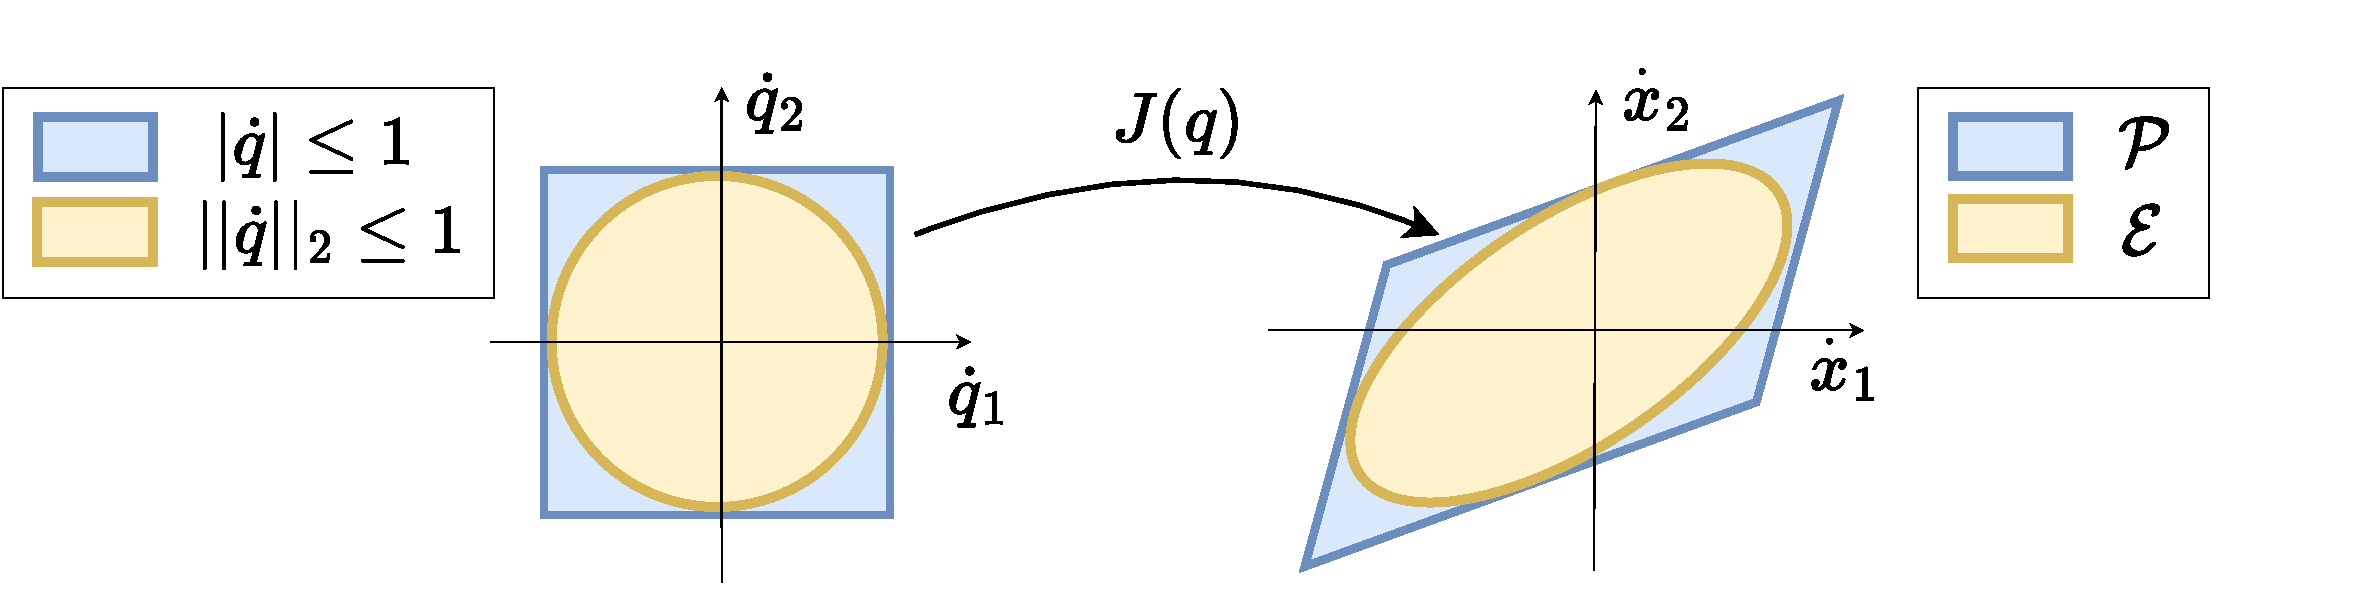
\includegraphics[width=0.7\textwidth]{Chapters/imgs/ellip_poly.pdf}
    \caption{An example manipulability polytope and ellipsoid geometry for a planar $m=2$ robot with $n=2$. The difference between the joint space limits for ellipsoid described with $||\dot{\bm{q}}||_2\leq1$ (orange) and the range limits $\bm{-1}\leq\dot{\bm{q}}\leq\bm{1}$ (blue) is shown on the right. The difference in obtained achievable task space velocity $\dot{\bm{x}}$ polytope $\mathcal{P}$ (blue) and ellipsoid $\mathcal{E}$ (orange) is shown on the right plot. The plots show that both in joint and task space the ellipsoid metric is an underestimation of the true robot's capacity.}
    \label{fig:ellip_poly_dif}
\end{figure}

Once the true robotic actuator limits are considered, the representation of physical abilities becomes convex polytope shaped. As opposed to the manipulability ellipsoid $\mathcal{E}$, manipulability polytope can be defined as
\begin{equation}
    \mathcal{P}(\bm{q}) = \left\{ \dot{\bm{x}} ~|~ \dot{\bm{x}} = J(\bm{q})\dot{\bm{q}},~~ \dot{\bm{q}}_{min}\leq\dot{\bm{q}} \leq \dot{\bm{q}}_{max} \right\}
\end{equation}
The manipulability polytope $\mathcal{P}$ represents an exact solution of the robot's task space velocity capacity, given robot's state $\bm{q}$
and its joint velocity limits $\dot{\bm{q}}$. The difference between the manipulability ellipsoid $\mathcal{E}$ and polytope $\mathcal{P}$ is shown for a simple 2d example on Figure \ref{fig:ellip_poly_dif}.
Polytope based physical ability metrics are the most complete local representation of task space physical abilities of robotic systems and they are used to characterise many task related physical values such as velocities \cite{Lee1997manip, long_constrained_2020}, forces \cite{chiacchio_evaluation_1996}, accelerations \cite{chiacchio_2000}, stiffness \cite{ajoudani2015role}, positioning accuracy \cite{pholsiri2005real}, etc.
The main downside to the polytope based metrics with respect to the ellipsoid based metrics is their computational complexity, making their use somewhat limited to non time critical applications.
% \todos{say that most of the stuff done with other metrics can be done with polytopes as well}

% \todos{
% \begin{itemize}
%     \item for robotics
%     \begin{itemize}
%         \item used to evaluate the robot capacity to execute certain tasks
%         \item to design more capable robots
%         \begin{itemize}
%             \item different visual metrics cable of being used to guarantee stuff
%             \item usually calculated in advance for the whole robot workspace 
%             \item payload for example, or reachable workspace, or wrench closure workspace for parallel robots
%             \item typically not taking in consideration robot's dynamics
%         \end{itemize}
%         \item to exploit robot's full potential when controlling it (or planning its movements)
%         \begin{itemize}
%             \item used in optimisation
%             \item different scalar metrics that are easy to calculate in real time
%             \item manipulability index, and all the other indexes from the overview paper
%             \item also ellipsoids were used for this to find the directions with max movement capacity
%         \end{itemize}        
%     \end{itemize}        
% \end{itemize}
% }

\subsection{Metrics for humans}

Evaluating physical abilities of humans is a much more challenging than for robotic systems, as human bodies are much more complicated systems that depend both on biological and biomechanical, as well as cognitive and psychological factors.

Measuring different physical abilities of human subjects is traditionally done experimentally. The ability of human subjects to achieve different physical quantities such as generate forces \cite{HODDER2016Testing,HOLZBAUR20072442}, reach positions \cite{CASTRO2019108}, execute movements \cite{Jessop2016} or generate stiffnesses \cite{Tsuji1995,Artemiadis2010}, is tested in laboratory environment for a set of predefined human postures or movements. These experiments enable finding precise physical abilities of one or multiple subjects, for the tested motions and postures.  Such experimental analysis are common tools for evaluation of physical abilities in sports \cite{Jessop2016}, where the motions and postures of interest are usually well define, and in rehabilitation \cite{HAISMA2006741} where the aim is to measure the progress of the human subject's recovery. However due to the large variability in human bodies and movements, it is challenging to generalise these results to the human subjects who were not part of the experiments, as well as to different postures and movements, of the same human subjects, that were not tested in the experiments.

In more varied and unstructured settings, where the human postures and movements are harder to characterise, such as in factory setting, the experimental metrics are impractical. For these scenarios, instead of characterising the physical ability of human subject directly, different metrics are developed aiming to evaluate the ergonomics of human postures and movements when executing tasks. These metrics are able to account for variations in human body anthropomorphic structure as well as for different movement and forces generation requirements of the tasks. Such metrics are often defined in a form of standards, such as \textit{Rapid Entire Body Assessment} (REBA) \cite{reba}, \textit{Rapid Upper Limb Assessment} (RULA) \cite{rula} or DULA and DEBA \cite{Yazdani2022} ( their differentiable equivalents), and manuals, such as Great Britain's \textit{Manual Handling Operation Regulations} \cite{health1992manual} or NASA's \textit{Man-systems integration standards} \cite{nasa}. These metrics are designed to give a certain score or a recommendation for the human postures, movements or force generation requirements of the task, in order to evaluate if the task is well suited for human's physical abilities. Common applications of these metrics, in factory settings, have for a goal to evaluate and improve the ergonomics of human's tasks \cite{Busch2017} and workplace layouts\cite{ORE20161, Lietaert2019}. However, these metrics, in order to be task and human subject agnostic, make coarse approximations of human physical abilities which are constraining when it comes to the online human robot collaboration scenarios\cite{maurice2015}. 
%\todo{motivate better, a sentence about problems} 

In order to characterise human's physical abilities, more finely, without the need for time consuming and impractical experimental evaluation, different metrics based on human musculoskeletal models are proposed. Human musculoskeletal models are relatively complete models of human bodies capable of describing different human body's biological and biomechanical parameters as well as its rigid body dynamics. Musculoskeletal models are actuated by muscle-tendon units, capable of applying a range of contracting forces, accelerations and velocities. Similar to robotic systems, several global and local physical ability metrics, based on musculoskeletal models, can be calculated by evaluating how different limits of the muscles as actuators effect human's task related physical abilities, such as to generate forces or motions. 

Several global physical ability metrics based on musculoskeletal models are introduced in literature, such as human upper extremity reachable workspace \cite{Lenarcic1994,Kurillo2013} or comfortable reachable workspace \cite{Figueredo2021}, the comfortablility map of the reachable workspace of human's upper limbs evaluated using RULA and REBA ergonomics scores. In addition to the global metrics many robotics inspired local, state dependent, metrics have been developed as well. Different authors have used their ellipsoid based representations to asses the velocity (manipulability) \cite{Rezzoug2012manipulability}, force \cite{rezzoug_application_2012, lazinica_higher_2010}, acceleration \cite{khatib2009robotics} and stiffness \cite{Artemiadis2010} capacity of humans based on their musculoskeletal models. Several of these ellipsoids have been extend to the more complete polytope representation as well, such as force polytope \cite{sasaki2011vertex, rezzoug_application_2012, carmichael_estimating_2013} and acceleration capacity polytope \cite{khatib2009robotics, demircan2012muscle}. As in the case of robotic systems, polytope based represents the exact solution to the physical ability evaluation, given an appropriate musculoskeletal model. However, as the musculoskeleral models are only an approximation of the true physics of human bodies the accuracy of the calculated physical ability metrics relies entirely on the correspondence between the model and the human subject. Multiple experimental studies were conducted on for the human upper limb force generation capacity, by Rezzoug et al. \cite{biomechanics1010008}, Hernandez et. al \cite{HERNANDEZ2015} as well as Sasaki et al. \cite{lazinica_higher_2010}, where the experimental results were compared to the force capacity polytope and ellipsoid representations. Their results confirm that the polytopes correspond better to the experimentally obtained capacity of the human subjects. However, the results further underline the importance of having an appropriate musculoskeletal model of the human subject. Even though many strategies have been developed for fitting the musculoskeletal models to human subjects in the biomechanics literature mostly based on different forms of scaling \cite{Lund2015, Ziyun2019}, it is still an open field of research. 

With the assumption of an appropriate and well adapted human musculoskeletal model of the human subject, polytopes and ellipsoids present an accurate estimation of the human's task related physical abilities. 
Even though polytopes are more accurate estimation, ellipsoid based representations, due to their computational efficiency, are still a preferred choice when it comes to evaluating human's physical ability, especially in real time applications. The difference in computational complexity between polytope and ellipsoid evaluation for musculoskeletal models is even more exaggerated than for the robotic systems. As the musculoskeletal models often have many muscles (often more than 50) final polytope geometry becomes complex which ultimately has a negative impact of their computation time.

% \todos{
% \begin{itemize}
%     \item for humans
%     \begin{itemize}
%         \item for humans the metrics are mush less exact, mostly empirical
%         \begin{itemize}
%             \item in labs
%             \item per subject
%             \item hard to generalize
%             \item takes time
%         \end{itemize}
%         \item simpler metrics 
%         \item used to evaluate the ergonomics of the human posture, his task or his workspace
%         \begin{itemize}
%             \item evaluated in-situ
%             \item different score based scalar metrics
%             \item ergonomics scores based on different metrics and manuals
%             \item rula, reba, payload manual, nasa and similar
%         \end{itemize}        
%         \item different set of metrics based on human miscalculate models
%         \item based on exact evaluation of different metrics (similar to robots)
%         \begin{itemize}
%             \item used to evaluate maximal human capacities
%             \item more or less all the metrics as for robots can be used
%             \item ellipsoids and polytopes to evaluate the maximal force capacity
%         \end{itemize}   
%         \item there are also those who try to combine the two
%         \item standards + musculoskeletal stuff
%         \begin{itemize}
%             \item comfortability metrics ( a combination of the two ) \cite{Figueredo2021}
%             \item however calculated in advance and relatively complicated to use, no dynamics
%         \end{itemize}   
%     \end{itemize}
    
% \end{itemize}
% }

\subsection{Physical abilities in human-robot collaboration}

Human's and robot's individual physical ability metrics have been used in different human-robot collaboration scenarios. Robot's physical abilities are often calculated in order to make sure that the task requirements comply with the robot's capacity, while human's physical ability and ergonomics metrics are then used to design the suitable robot behavior in order to make the human's task and posture more ergonomic. Such collaboration strategies consider the robot be an action vector with limited resources whose job is to improve the task performance and the human ergonomics at the same time. Examples of such human-centered collaborative scenarios are described by Kim et al. \cite{KIM2021102084}, where the robot adapts the position of the manipulated object in space in order to improve human's ergonomics, or in the context of exoskeleton control by Carmichael et al. \cite{carmichael2013admittance,carmichael_towards_2011} and Pertic et al. \cite{petric2019assistive}, where the robot adapts to different assistance needs of the human operator.

However, when it comes to the human-robot collaboration scenarios where a human and a robot interact physically in order to execute a certain task, characterising their joint physical abilities is still an open research question. Human and robot physical abilities are often expressed in different ways, with different units and with fundamentally different metrics, making the procedure of combining them challenging. Therefore, in order to characterise their joint physical capacity, the first step is to express their individual physical abilities need in the same unified form. 

When it comes to multi-robot physical collaboration, Chiacchio et al. \cite{chiacchio_global_1991} have shown that ellipsoid based metrics can be used to calculate their combined joint velocity (manipulability) capacity. The final joint capacity has an ellipsoid form as well.  However, in their formulation, the collaboration of multiple robots is essentially seen as one larger robot, combining all the joints of all the robots, resulting in the robot with $n=n_1 + n_2 + \ldots$ joints.
\begin{equation}
    \bm{q} = \begin{bmatrix}
        \bm{q}_1\\ \bm{q}_2 \\ \ldots
    \end{bmatrix}, \quad
    \dot{\bm{q}} = \begin{bmatrix}
        \dot{\bm{q}}_1\\\dot{\bm{q}}_2 \\ \ldots
    \end{bmatrix}, \quad
    J(\bm{q}) = \text{diag}([J_1(\bm{q}_1),~ J_2(\bm{q}_2),~\ldots])
\end{equation} 
Where $n_i$ is the number of joints, while $\bm{q}_i$ is the vector of joint positions and $J_i(\bm{q}_i)$ is the jacobian matrix for each one of the robot's involved.

\begin{figure}[!h]
    \centering
    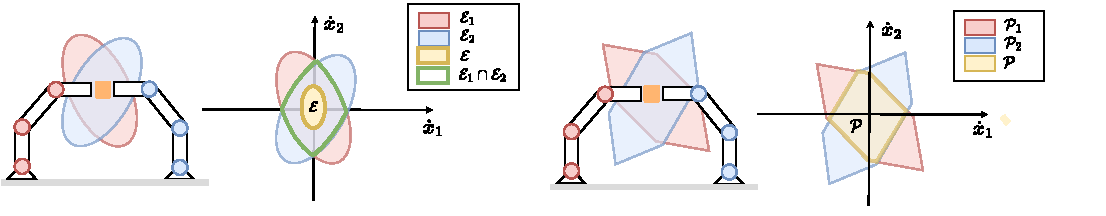
\includegraphics[width=1.05\linewidth]{Chapters/imgs/collab_manip_poly.pdf}
    \caption{Comparison of using ellipsoids (left) and polytopes (right) for collaborative physical ability calculation. Using polytopes, the common velocity capacity of the two robots is calculated as the intersection of their polytopes $\mathcal{P}=\mathcal{P}_1 \cap \mathcal{P}_2$. In ellipsoid case the intersection of the ellipsoids (green) is no longer an ellipsoid and it is hard to characterise, while the collaborative ellipsoid $\mathcal{E}$ (orange) introduced by Chiachio et al. \cite{chiacchio_global_1991} is a large underestimation of the true joint capacity.}
    \label{fig:collab_mani_poly}
\end{figure}
With such large number of joints, the euclidean norm $||.||_2$ limits present a large under-approximation of the real robot's limits, resulting in large under-approximation of the true capacity of the collaboration. As shown on the example on Figure \ref{fig:collab_mani_poly}, a more precise approach would be to intersect the ellipsoids calculated independently for all the robots $$\mathcal{E}=\mathcal{E}_1 \cap \mathcal{E}_2  \cap \ldots$$ However, the intersection operation over ellipsoids is hard to characterise and to evaluate, as the intersection of two ellipsoid is no longer an ellipsoid, and even if the intersection of the ellipsoids is obtained, it is just an approximation of true common capacity. 

Expressing the robot's physical ability in the polytope form however is not just the exact solution, but enables using the polytope algebra to do different operations, such as sum, intersection and convex-hull. These operations are well defined and can be calculated efficiently. The work from Jihong Lee \cite{lee2001velocity} shows that polytopes metrics can be used to describe the common velocity capacity of multi-arm collaborative robotic system.  The work describes an efficient way of calculating the joint velocity capacity by intersecting the individual polytopes of each one of the robots involved, resulting in a convex polytope shaped joint velocity capacity $$\mathcal{P}=\mathcal{P}_1 \cap \mathcal{P}_2  \cap \ldots$$
By exploiting different polytope algebra operations it is possible to express different physical collaboration scenarios as well. For example, if now the robots would be re-arranged from the parallel to the serial configuration, where the robot would be stacked one on top of the other, their joint velocity capacity would correspond to the Minkowski sum of their individual capacity $$\mathcal{P}=\mathcal{P}_1 \oplus \mathcal{P}_2  \oplus \ldots$$

\begin{figure}[!h]
    \centering
    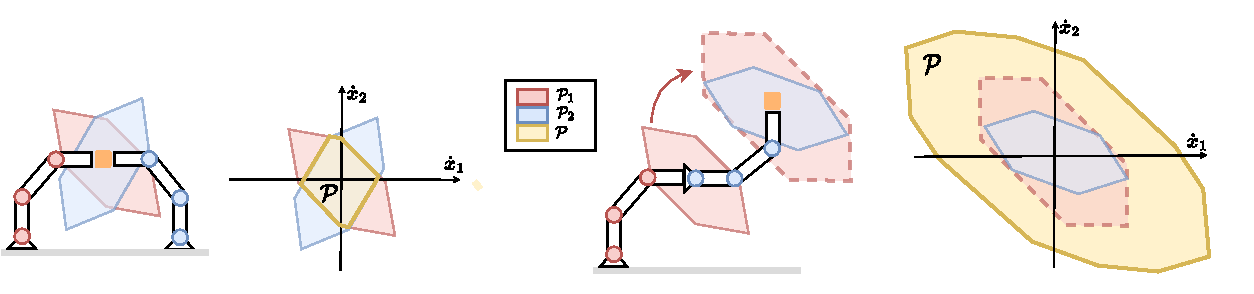
\includegraphics[width=\linewidth]{Chapters/imgs/collab_serial_parallel.pdf}
    \caption{Two examples of using polytope based metrics for joint achievable velocity capacity calculation of multiple robots collaborating. Figure on the left shows the parallel collaboration where the common capacity is calculated with the intersection. Figure on the right shows the serial collaboration where the common capacity is a Minkowski sum of their individual capacity. As the capacity is calculated at the end-effector of the second robot, the velocity polytope $\mathcal{P}_1$ of the first robot has to be transformed the same position (in red dashed border).}
    \label{fig:collab_serial_parallel}
\end{figure}
Figure \ref{fig:collab_serial_parallel} shows a simplified plannar example of the joint velocity capacity calculation for parallel and serial robot arrangement.

In summary, the polytope representation enables the physical abilities of robots, humans, and their collaboration to be expressed through a unified format. Furthermore, as many different physical abilities of humans and robots can be expressed in polytope form, it has the potential to provide an important set of tools for evaluating different collaboration tasks.
For example, by evaluating different physical abilities relevant to the task, it enables characterising if the task is more suitable for humans, robots or for different modes of their physical collaboration.  


% \todos{
% \begin{itemize}
%     \item what about collaboration metrics
%     \item Some metrics have been used but still very limited
%     \item when it comes to characterising their common capacity
%     \begin{itemize}
%         \item payload metrics might be used - very limiting
%         \item and ellipsoid based stuff from chiacchio - robots
%         \item lee also with polytopes a bit - robots
%         \item we still lack proper metrics to unify the humans and robots
%         \item they are usually expressed in different ways and hard to combine
%     \end{itemize}
%     \item Different ways of enhancing collaboration using physical ability metrics
%     \begin{itemize}
%         \item Collaborative workspace design for example - vincent paper
%         \item visualisation to the user 
%         \item Communicate the current robot state to the operator when collaborating
%         \item assist as needed control of exoskeletons also maybe (ellipsoids petric + polytopes carmichael)
%         \item but still not considering robot's capacity - robot only adapts to the human needs
%     \end{itemize}
% \end{itemize}
% }


\subsection{Why polytopes?}

As described in the previous sections, polytope representation of physical abilities accurately 
characterises the physical abilities of robotic manipulators, at the same time being the most complete approximation of human physical abilities based on musculoskeletal models. Additionally, since most of the well known polytope formulations for robotic systems can be formulated as polytopes for musculoskeletal models as well, they enable evaluating and comparing human's and robot's physical abilities in a unified manner. Furthermore, the polytope algebra enables operations over multiple polytopes and, in that way, has a potential to enable characterising common physical abilities of humans and robots involved in different physical collaboration scenarios. 

When it comes to using polytopes in practical applications, there are two standard ways of representing them: as a set of vertices (vertex representation) or as a set of inequality constraints corresponding to its faces (half-plane representation) \cite{fukuda2004frequently}. Transforming a polytope into these standard representations enables using different efficient tools from computational geometry and polytope algebra in order to do operations over polytopes, for example find minimal distance between polytopes \cite{Ong1997gjk}, polytope volume \cite{Lawrence1991Volume} or calculate the convex hulls \cite{Barber1996}, Minkowski sums \cite{BARKI2009525}, intersections and unions of multiple polytopes \cite{Tiwary2008}. Additionally, it opens doors for different simplification strategies of polytopes, by finding the inner and outer approximations of polytopes using spheres \cite{Botkin1994} or cubes \cite{BEMPORAD2004151}.

Furthermore, as discussed by Finotello et al. \cite{Finotello1998}, polytopes enable calculating many other local different performance metrics, such as Maximum Available Value (MAV) corresponding to the highest achievable magnitude of the task space variable (velocity, acceleration, force, static error, etc.), Maximal Isotropic Value (MIV) corresponding to the maximal value achievable in all the directions in space or Directional Index (DI) \cite{boschetti_minto_2023} corresponding to the maximum achievable task space variable in certain direction in space or calculating. Additionally, polytope volume and major (preferred) axis can be used as performance metrics as well \cite{chiacchio_global_1991, Long2018Evaluating}.

In case of characterising physical abilities, transforming the polytopes to the vertex representation enables using efficient triangulation algorithms from computational geometry. Most of the standard visualisation tools can visualise such triangulated meshes in very efficient manner, even in real time. 
In the context of human-robot collaboration, an example application of polytope visualisation was proposed by Zolotas et al. \cite{Zolotas2021}, where the robot's velocity polytopes were used to inform the operator about the robot's movement capacity during the teleportation task. Similar application was recently proposed by Weistroffer et al. \cite{Weistroffer2022Using}, where the polytopes of robot's force capacity were visualised to the operator designing the collaborative workspace with the aim to improve its safety and ergonomics. 

Polytopes can be expressed as a set of linear inequalities $A\bm{x}\leq\bm{b}$, that can be integrated into different optimisation problems in a form of linear inequality constraints. Most of the standard Quadratic Programming (QP) \cite{boggs_tolle_1995} and Linear Programming (LP) \cite{GOLDFARB198973} solvers support the inequality constraints in an efficient manner. A typical example applications often based on different optimisation strategies are robot control and trajectory planning applications. In the context of human-robot collaboration, being able to consider both robot's and human's physical abilities with in those contexts, opens doors for creating more human-centred robot control (or trajectory planning) strategies where robot's behaviour is adapted (planned), not just with respect to its own physical abilities, but also to the ones of the human.
Potential benefits of considering human's physical abilities for creating human-centred robot control were demonstrated in the context of assistive exoskeletons. In these scenarios, the robot provides the assistance to the operator adapted to his current physical ability, so called \textit{Assist As Needed} (AAN)\cite{carmichael2013admittance} control paradigm.
However, as the polytope representation of human physical abilities based on musculoskeletal models results in a highly complex computational problem to solve, in order to be used in real-time applications, so far all solutions proposed in the literature use different approximations of human's physical abilities. In the work by Carmichael et al. \cite{carmichael_towards_2011}, a coarse approximation of human's force capacity was used, Aldini et al.\cite{Aldini2021RealTime} have used a learning based approach to estimate human's force ability using polynomial fitting, while in the work by Petric et al.\cite{petric2019assistive}, similar strategy was used where human's force abilities were approximated using ellipsoids.

Therefore, polytope representation provides an accurate representation of both humans' and robots' physical abilities in a unified manner. Additionally, it enables characterising the common physical abilities of humans and robots interacting physically when executing certain task as well. Representing these capacities in the polytope form enables using many efficient tools form the polytope algebra and computational geometry to perform operations over polytopes and to extract useful information concerning the tasl, for example different performance indicators. Additionally, polytopes can be transformed to more standard forms such as a set of vertices or set of inequalities which can then be used with standard visualisation tools and integrated in different optimisation problems, opening many doors in human-robot collaborative applications.

This chapter further brings an overview of common polytope formulations for characterising different physical abilities of robots in section \ref{ch:robot_metrics} and humans in section \ref{ch:human_metrics}. Section \ref{ch:collab_metrics} then discusses combining their individual polytopes using polytope algebra, in order to characterise their common physical abilities when interacting physically in the context of the object manipulation. Finally, section \ref{ch:collab_metrics_overview} brings the structured view on the introduced polytope formulations and their use in characterising the human-robot interaction abilities.


% \todos{
% \begin{itemize}
%     \item polytope based metrics might be able to close the gap
%     \item in our opinion the best ones - unifying most of the other metrics
%     \item exact solution 
%     \item encapsulate many of the other metrics inside (volume, direction of maximal magnitude, singularity, ....)
%     \item can be easily visualised
%     \item defined both for robots and humans (based on musculoskeletal models)
%     \item can be used in optimisation
%     \item operation over polytopes (sum, intersection convex-hull) well defined as opposed to the other metrics
% \end{itemize}
% }
\section{Polytope representation of physical abilities}
\label{ch:poly_metrics}
Physical ability characterisations based on polytopes are numerous in the literature, therefore the aim of this section is to provide an overview of common polytope formulations for different physical abilities of robotic systems and humans, based on their musculoskeletal models. Additionally, section \ref{ch:collab_metrics} demonstrates the use of polytopes to calculate the physical abilities in collaborative scenarios. Finally, section \ref{ch:which_metric_which} brings the categorisation of the common polytope formulations with respect to the nature of their formulation.

\subsection{Robotic manipulators}
\label{ch:robot_metrics}

Physical ability characterisations based on polytopes are most accurate local, state dependent, metrics for the performance analysis of robotic systems \cite{pholsiri2005real,Finotello1998}. They describe a mapping between the robot's actuator limits (torques, accelerations , velocities, etc.) and the limits of different task space variables (wrenches, accelerations, velocities, etc.) . 

The aim of this section is to provide an overview of common polytope formulations for robotic systems in an unified view.  Therefore, section \ref{ch:robot_dyn_kin} beings a quick overview of the dynamics and kinematics equations for robotic systems, used for different polytope definitions. Definitions 
of common polytope characterisations of physical abilities are then described in subsequent chapters.

\subsubsection{Dynamics and kinematics relationships}
\label{ch:robot_dyn_kin}
The actuation limits, of a robotic manipulator with $n$ joints, are commonly specified as independent ranges of achievable actuator positions $\bm{q}\in \mathbb{R}^n$, velocities $\dot{\bm{q}}\in \mathbb{R}^n$, actuator torques $\bm{\tau}\in \mathbb{R}^n$ and sometimes even torque derivative $\dot{\bm{\tau}}\in \mathbb{R}^n$.
\begin{subequations}
\begin{align}
\bm{q} &\in [ {\bm{q}}_{min}, {\bm{q}}_{max}], \quad\dot{\bm{q}} \in [\dot{\bm{q}}_{min},  \dot{\bm{q}}_{max}], \\
\quad\bm{\tau} &\in [\bm{\tau}_{min},  \bm{\tau}_{max}],
\quad\dot{\bm{\tau}} \in [\dot{\bm{\tau}}_{min},  \dot{\bm{\tau}}_{max}] \label{eq:dyn_limits:torque}
\end{align}
\label{eq:dyn_limits}
\end{subequations}
The dynamical model, of a standard serial robotic manipulator with a fixed base, is commonly defined as
\begin{equation}
M(\bm{q})\ddot{\bm{q}} + C(\bm{q},\dot{\bm{q}})\dot{\bm{q}} + \bm{g}(\bm{q}) + J^T(\bm{q})\bm{f} = \bm{\tau} 
\label{eq:dyn_model_rob}
\end{equation}
where $M(\bm{q}) \in \mathbb{R}^{n \times n}$ and $C(\bm{q},\dot{\bm{q}})\in \mathbb{R}^{n \times n}$ are its inertia and Coriolis matrices, $\bm{g} (\bm{q})\in \mathbb{R}^n$ is the state dependent gravity vector, $J(\bm{q}) \in \mathbb{R}^{m\times n}$ is the state dependant jacobian matrix, $\bm{f}\in \mathbb{R}^m $ is the vector of applied external wrenches and $\bm{q},\dot{\bm{q}},\ddot{\bm{q}}$ are robot's joint positions, velocities and accelerations respectively.

Furthermore, the mapping between the $n$ dimensional space of robot's actuator (joint) positions $\bm{q}\in \mathbb{R}^n$ and the $m$ dimensional task space positions $\bm{x} \in \mathbb{R}^m$ can be found through the robot's forward kinematics 
\begin{equation}
    \bm{x} = f_{fk} (\bm{q})
\end{equation}
whereas the task space velocity $\dot{\bm{x}}\in \mathbb{R}^m$, acceleration $\ddot{\bm{x}}\in \mathbb{R}^m$ and jerk $\dddot{\bm{x}}\in \mathbb{R}^m$ can be found through the state dependent  $\{\bm{q},\dot{\bm{q}},\ddot{\bm{q}}\}$  and nonlinear mapping
\begin{subequations}
\begin{align}
\dot{\bm{x}}&= {J}(\bm{q})\dot{\bm{q}} \label{eq:js_to_cs_vaj:vel}\\
\ddot{\bm{x}}&= J(\bm{q})\ddot{\bm{q}} + \dot{J}(\bm{q},\dot{\bm{q}})\dot{\bm{q}} \label{eq:js_to_cs_vaj:accel}\\
\dddot{\bm{x}}&= J(\bm{q})\dddot{\bm{q}} + 2\dot{J}(\bm{q},\dot{\bm{q}})\ddot{\bm{q}} + \ddot{J}(\bm{q},\dot{\bm{q}},\ddot{\bm{q}})\dot{\bm{q}}\label{eq:js_to_cs_vaj:jerk}
 \end{align} \label{eq:js_to_cs_vaj}
\end{subequations}
were $J(\bm{q}) $ is the jacobian matrix
\begin{equation}
    J(\bm{q}) = \frac{\partial f_{fk} (\bm{q})}{\partial \bm{q}}
\end{equation}
while $\dot{J}(\bm{q},\dot{\bm{q}})$ and $\ddot{J}(\bm{q},\dot{\bm{q}},\ddot{\bm{q}})$ are its first and second time derivatives.


It is worth noting that in general case, $m$ dimensional task space might include positions and orientations, for example if the task space corresponds to the Cartesian space, where $m=6$. When the task space includes orientations, the task space pose (including the position and orientation) is often expressed is the homogeneous matrix form $\bm{x}\in SE(3)$. Then the task space velocity vector $\dot{\bm{x}}\in\mathbb{R}^6$ becomes the Cartesian space \textit{twist vector} $\bm{\nu}$, expressing the translation and rotation velocity at the same time. However, in such cases, the twist $\bm{\nu}$ does no longer correspond to the time derivative of the task space pose $\bm{\nu}\neq\frac{d\bm{x}}{dt}$. Despite this distinction, for simplicity reasons, this work uses the notation $\dot{\bm{x}}$, $\ddot{\bm{x}}$, and $\dddot{\bm{x}}$ to represent velocity, acceleration, and jerk of the task space variables, respectively.

When considering certain fixed robot state $\{\bm{q},\dot{\bm{q}},\ddot{\bm{q}}\}$, robot's dynamical model (\ref{eq:dyn_model_rob}) and the joint to task space mapping (\ref{eq:js_to_cs_vaj}) become linear, as the state dependent matrices become fixed. Using these linear and affine mappings the achievable sets of different task space variables (ex. velocity $\dot{\bm{x}}$, accelerations $\ddot{\bm{x}}$ or wrenches $\bm{f}$), given the range of robot's actuator limits (\ref{eq:dyn_limits}), can be found through the equations (\ref{eq:dyn_model_rob}) and (\ref{eq:js_to_cs_vaj}). The obtained achievable sets then have a form of convex polytopes as the mapping between the robot limits and the task space variables is linear.


\paragraph*{Kinematic joint limits} As a precise robot's dynamical model is sometimes hard to obtain, instead of specifying the actuator torque limits (\ref{eq:dyn_limits:torque}), the manufacturers often rather specify robot's actuator limits in a kinematic form, considering them to have limited and constant acceleration $\ddot{\bm{q}} \in \mathbb{R}^n$ and jerk $\dddot{\bm{q}} \in \mathbb{R}^n$ limits.
\begin{equation}
\ddot{\bm{q}} \in [\ddot{\bm{q}}_{min}, \ddot{\bm{q}}_{max}], ~~ \dddot{\bm{q}} \in [ \dddot{\bm{q}}_{min}, \dddot{\bm{q}}_{max}] 
\label{eq:kin_limits}
\end{equation}
Using these kinematic actuator limits, the linearisation procedure of the mapping (\ref{eq:js_to_cs_vaj}) around given robot state $\{\bm{q},\dot{\bm{q}},\ddot{\bm{q}}\}$, can then be used to obtain the polytope shaped achievable sets of kinematic task space variables (ex. velocity $\dot{\bm{x}}$, acceleration $\ddot{\bm{x}}$, jerk $\dddot{\bm{x}}$).



\paragraph*{} Many well known polytope formulations for characterising the physical abilities of robotic manipulators are proposed in the literature, characterising the influence of robots dynamics (\ref{eq:dyn_limits}) and kinematics joint limits (\ref{eq:kin_limits}) on the task space variables through its linearised dynamics (\ref{eq:dyn_model_rob}) and kinematics (\ref{eq:js_to_cs_vaj}) equations. Some of the most common polytope formulations are listed in the following sections.

\subsubsection{Velocity polytope}
\label{ch:vel_poly}

Achievable task space velocity capacity is a common physical ability metric for robotic manipulators describing its ability to generate task space velocities $\dot{\bm{x}}$ in different directions in space, given its joins space velocity $\dot{\bm{q}}$ limits. Robot's velocity capacity is commonly know as its manipulability or dexterity capacity as well. This metric has been first introduced by Yoshikawa \cite{yoshikawa_manipulability_1985} in the ellipsoid form and later extended to the polytope form \cite{chiacchio_global_1991, Lee1997manip}. %\todo{try finding the paper: 
%"Kinetostatic performance limits of cooperating robot manipulators using force-velocity polytopes"
%}

For any fixed robot configuration $\bm{q}$ the ranges of joint velocity limits 
\begin{equation}
   \dot{\bm{q}}\in\left[\dot{\bm{q}}_{min}, \dot{\bm{q}}_{max} \right]
\end{equation}
can be projected to the $m$ dimensional task space using the jacobian matrix $J(\bm{q})$, obtaining the convex polytope of achievable task space velocities  
\begin{equation}
    \mathcal{P}_v(\bm{q}) = \left\{ \dot{\bm{x}} \in \mathbb{R}^m ~|~ \dot{\bm{q}}\in\left[\dot{\bm{q}}_{min}, \dot{\bm{q}}_{max} \right], ~~ \dot{\bm{x}} = J(\bm{q})\dot{\bm{q}} \right\}
    \label{eq:poly_vel_rob}
\end{equation}

Velocity capacity metrics are important tools for evaluating robot's movement capacity in different directions in space for a given configuration $\bm{q}$, while the polytope form is their exact representation. Different variants of polytope formulations are commonly used for robot redundancy resolution, by finding the robot configurations that maximise the robot's movement capacity and avoid singular positions\cite{Marani2002,Thygeson2017}, which can be seen as a zero velocity capacity in certain directions in space \cite{merlet_jacobian_2006}.  They have also been used for path planning \cite{Pardi2020,Nagatani2002} and object grasping \cite{Fei2019,XU2021300}. 

The polytope representation though is less commonly used in time-critical applications, due to their computational complexity. However, Long et al. have shown that polytopes can be used for whole body humanoid robot control \cite{long_constrained_2020} in real-time. Recently, Zolotas et al. have shown their potential to be used for real-time visualisation to the user in the case of robot teleportation \cite{Zolotas2021}. 

\subsubsection{Kinematic Acceleration and Jerk polytope}\label{ch:kin_accel_jerk}
In a similar manner to the achievable velocity polytope $\mathcal{P}_v$, the achievable task space acceleration $\ddot{\bm{x}}$ and jerk $\dddot{\bm{x}}$ sets can be expressed using the kinematic mapping (\ref{eq:js_to_cs_vaj}). 

Given the limits of the actuator accelerations $\ddot{\bm{q}}$ and a given robot state $\{\bm{q},\dot{\bm{q}}\}$, the achievable polytope $\mathcal{P}_a$ of task space accelerations $\ddot{\bm{x}}$ can be found using the mapping (\ref{eq:js_to_cs_vaj:accel}).
\begin{equation}
    \mathcal{P}_a(\bm{q}, \dot{\bm{q}}) = \left\{ \ddot{\bm{x}} \in \mathbb{R}^m ~|~ \ddot{\bm{q}}\in\left[\ddot{\bm{q}}_{min}, \ddot{\bm{q}}_{max} \right], ~~ \ddot{\bm{x}} = J(\bm{q})\ddot{\bm{q}} + \bm{a}_b(\bm{q}, \dot{\bm{q}})  \right\}
    \label{eq:poly_accel_kin}
\end{equation}
where $\bm{a}_b(\bm{q}, \dot{\bm{q}})$ is considered as a constant bias term for any given robot state $\{\bm{q},\dot{\bm{q}}\}$
\begin{equation}
    \bm{a}_b(\bm{q}, \dot{\bm{q}}) = \dot{J}(\bm{q},\dot{\bm{q}})\dot{\bm{q}}
\end{equation}.

The achievable task space jerk polytope $\mathcal{P}_j$ can be found for any given robot state $\{\bm{q},\dot{\bm{q}},\ddot{\bm{q}}\}$, by considering a limited range of actuator jerks $\dddot{\bm{q}}$ and using the mapping (\ref{eq:js_to_cs_vaj:jerk})
\begin{equation}
    \mathcal{P}_j(\bm{q}, \dot{\bm{q}}, \ddot{\bm{q}}) = \left\{ \dddot{\bm{x}} \in \mathbb{R}^m ~|~ \dddot{\bm{q}}\in\left[\dddot{\bm{q}}_{min}, \dddot{\bm{q}}_{max} \right], ~~ \dddot{\bm{x}} = J(\bm{q})\dddot{\bm{q}} + \bm{j}_b(\bm{q}, \dot{\bm{q}},\ddot{\bm{q}}) \right\}
    \label{eq:poly_jerk_kin}
\end{equation}
where $\bm{j}_b(\bm{q}, \dot{\bm{q}},\ddot{\bm{q}})$ is a constant bias term for any fixed robot state $\{\bm{q},\dot{\bm{q}},\ddot{\bm{q}}\}$
\begin{equation}
    \bm{j}_b(\bm{q}, \dot{\bm{q}},\ddot{\bm{q}}) =2\dot{J}(\bm{q},\dot{\bm{q}})\ddot{\bm{q}}+ \ddot{J}(\bm{q},\dot{\bm{q}},\ddot{\bm{q}})\dot{\bm{q}}
\end{equation}

An example application of the jerk and acceleration polytopes is described by Grandguillaume et al. where the polytopes are used to find the optimal tool orientation for 5-axis milling \cite{Grandguillaume2021}.

\subsubsection{Precision (maximal positioning error) polytope }

Robotic manipulators often have limited positioning precision of their actuators. Actuator precision depends on many different factors, such as position sensor used, motor gearing, motion control strategy etc \cite{pholsiri2005real,Finotello1998}. However, in most cases the manufacturers are able to provide the limits on the maximal positioning error for each of the actuators within a certain range
\begin{equation}
    \delta\bm{q} \in [\delta\bm{q}_{min}, \delta\bm{q}_{min}]
    \label{eq:pos_error}
\end{equation}

Depending on the robot's configuration $\bm{q}$ the actuator position error $\delta\bm{q}$ will produce different task space positioning errors, their relationship can be calculated through the kinematic mapping (\ref{eq:js_to_cs_vaj:vel})
\begin{equation}
    \delta\bm{x} = J(\bm{q})\delta \bm{q}
\end{equation}
where $\delta\bm{x}\in\mathbb{R}^m$, in general case presents both position and orientation error.

The limits of the task space positioning error $\delta \bm{x}$ in a certain robot configuration $\bm{q}$, given the limits (\ref{eq:pos_error}) specified by the manufacturer, can be expressed by a convex polytope $\mathcal{P}_\delta$
\begin{equation}
    \mathcal{P}_\delta(\bm{q}) = \left\{ \delta \bm{x} \in \mathbb{R}^m ~|~ \delta  {\bm{q}}\in\left[ \delta {\bm{q}}_{min}, \delta {\bm{q}}_{max} \right], ~~  \delta  {\bm{x}} = J(\bm{q}) \delta {\bm{q}} \right\}
    \label{eq:poly_precision_rob}
\end{equation}

\subsubsection{Wrench/Force polytope}
\label{ch:poly_force}
Task space force (or more generally wrench) capacity metric is one of the most well known physical capacity metrics for robotics manipulators alongside the velocity (manipulability) capacity. It has been first introduced by Chiacchio et al. \cite{chiacchio_evaluation_1996} in a form of an ellipsoid as well as in the polytope form.

This metric establishes the relationship between the robot's actuator torque limits $\bm{\tau}$ and the achievable set of the task space wrenches $\bm{f}$.
Given the robot's manipulators dynamics equation (\ref{eq:dyn_model_rob}) 
\begin{equation}
\underbrace{M(\bm{q})\ddot{\bm{q}} + C(\bm{q},\dot{\bm{q}})\dot{\bm{q}} + \bm{g}(\bm{q})}_{\bm{\tau}_b(\bm{q},\dot{\bm{q}},\ddot{\bm{q}})} + J^T(\bm{q})\bm{f} = \bm{\tau} 
\end{equation}
for any given robot state $\{\bm{q},\dot{\bm{q}}\}$, and given joint acceleration $\ddot{\bm{q}}$ to be achieved, the effects of the robot's motion and the gravity can be expressed as a constant torque vector $\bm{\tau}_b(\bm{q},\dot{\bm{q}},\ddot{\bm{q}})$. Then the polytope of achievable task space wrenches $\bm{f}$ can be expressed as
\begin{equation}
    \mathcal{P}_f(\bm{q},\dot{\bm{q}},\ddot{\bm{q}}) = \left\{ \bm{f} \in \mathbb{R}^m ~|~ \bm{\tau}\in\left[\bm{\tau}_{min}, \bm{\tau}_{max} \right], ~~ J^T(\bm{q})\bm{f} = \bm{\tau} -\bm{\tau}_b(\bm{q},\dot{\bm{q}},\ddot{\bm{q}}) \right\}
    \label{eq:poly_force_rob}
\end{equation}

If achievable wrench capacity $\mathcal{P}_f$ is evaluated in kinetostatic conditions $\dot{\bm{q}},\ddot{\bm{q}}\approx\bm{0}$, the torque bias vector $\bm{\tau}_b$ corresponds to the gravity vector $\bm{g}(\bm{q})$ 
\begin{equation}
    \bm{\tau}_b(\bm{q},\bm{0},\bm{0}) = \bm{g}(\bm{q})
\end{equation}

As wrench polytopes describe the feasible range of task space wrenches that the robot can apply in certain configuration, they can be used in many different analysis applications as a performance metric, as well as in robot control in order to guarantee that the task requirements are within robot's capacity. An example application of wrench capacity polytopes for performance analysis of robotic excavator is described by Zou et al. for \cite{Zou2019}. Ferrolho et al. \cite{ferrolho_residual_2020} have described the application of wrench polytopes in offline dynamic trajectory planning. On the other hand, the applications of wrench polytopes in real-time applications are less common, mostly due to their computational complexity. However, Orsolino et al. \cite{Orsolino2018} have recently showed the application of wrench polytopes in real-time control of legged robots.

\subsubsection{Acceleration polytope}
\label{ch:accel_poly_robot}

The kinematic acceleration capacity described in section \ref{ch:kin_accel_jerk} considers constant and independent acceleration capacity for each robot's actuator (\ref{eq:kin_limits}), however the true acceleration limits of the robot's actuators depend on their torque capacity (\ref{eq:dyn_limits}) as well as on the robot's inertia 
$M(\bm{q})$ which is highly configuration dependent. 

Given the robot's dynamics equations (\ref{eq:dyn_model_rob}) 
\begin{equation}
M(\bm{q})\ddot{\bm{q}} + \underbrace{C(\bm{q},\dot{\bm{q}})\dot{\bm{q}} + \bm{g}(\bm{q}) + J^T(\bm{q})\bm{f}}_{\bm{\tau}_b(\bm{q},\dot{\bm{q}},\bm{f}) } = \bm{\tau} 
\end{equation}
for any given robot state $\{\bm{q},\dot{\bm{q}}\}$ and applied external wrench $\bm{f}$, the effects of the robot's motion, the gravity as well as the applied external wrenches, can be grouped in a constant torque vector $\bm{\tau}_b(\bm{q},\dot{\bm{q}},\bm{f})$. Then the actuator acceleration $\bm{q}$ can be expressed in relationship to the applied joint torque $\bm{\tau}$
\begin{equation}
    \ddot{\bm{q}} = M(\bm{q})^{-1}\bm{\tau} - M(\bm{q})^{-1}\bm{\tau}_b(\bm{q},\dot{\bm{q}},\bm{f})
\end{equation}
Finally, the actuator accelerations $\ddot{\bm{q}}$ can be transformed to the task space using the mapping (\ref{eq:js_to_cs_vaj:accel})
\begin{equation}
    \ddot{\bm{x}} = J(\bm{q})M(\bm{q})^{-1}\bm{\tau} - \underbrace{J(\bm{q})M(\bm{q})^{-1}\bm{\tau}_b(\bm{q},\dot{\bm{q}},\bm{f}) + \dot{J}(\bm{q}, \dot{\bm{q}})\dot{\bm{q}}}_{\bm{a}_b(\bm{q},\dot{\bm{q}},\bm{f})}
\end{equation}
where $\bm{a}_b(\bm{q},\dot{\bm{q}},\bm{f})$ presents a constant bias vector for any fixed joint state $\{\bm{q},\dot{\bm{q}},\bm{f}\}$. The polytope $\mathcal{P}_a$ of achievable task space accelerations $\ddot{\bm{x}}$ can then be expressed as
\begin{equation}
    \mathcal{P}_a(\bm{q},\dot{\bm{q}},\bm{f}) = \left\{ \ddot{\bm{x}} \in \mathbb{R}^m ~|~ \bm{\tau}\in\left[\bm{\tau}_{min}, \bm{\tau}_{max} \right], ~ \ddot{\bm{x}} = J(\bm{q})M(\bm{q})^{-1}\bm{\tau} - \bm{a}_b(\bm{q},\dot{\bm{q}},\bm{f}) \right\}
    \label{eq:pol_accleration_rob}
\end{equation}

As opposed to the kinematic acceleration polytope (\ref{eq:poly_accel_kin}) described in section \ref{ch:kin_accel_jerk}, this formulation not only represents more realistic acceleration capacity but it is able to account for the effect of the robot's motion, the effects of the gravity as well as its potential payload etc. 

This metric has been initially introduced by Chiacchio \cite{chiacchio_2000} in the ellipsoid form and later extended to the polytope form by  Rosenstein and Grupen \cite{rosenstein2002velocity}. An application of this metric in off-line analysis has been proposed by Jang and Lee \cite{Jang2009}, using the acceleration polytopes to analyse and optimise multi-fingered object grasping. Acceleration polytopes are used in real-time robot control applications as well. For example, Jeong and Tsagarakis \cite{jeong2006optimal} proposed an application of acceleration polytopes for robotic manipulators in order to optimise the robot's braking characteristics in real-time and to reduce the impact forces. 

\subsubsection{Stiffness polytope}
\label{ch:robot_stiffness_poly}
A different well known task space physical ability metrics for robotic manipulators is related to impedance control. If a certain frame of the robotic manipulator (ex end-effector frame) is controlled to have a behaviour of virtual spring with the task space stiffness $K_c \in \mathbb{R}^{m\times m}$
\begin{equation}
    \bm{f} = K_c \Delta\bm{x}
\end{equation}
where $\bm{f}\in\mathbb{R}^m$ is the  external wrench applied to the robot (by the environment or a human operator), and the $\Delta \bm{x}\in\mathbb{R}^m$ is the resulting displacement corresponding to the virtual spring with the square, $m\times m$, stiffness matrix $K_c$, where $m$ is the task space dimension.  In case of standard impedance control for a robotic manipulator in Cartesian space, controlling both position and orientation ($m=6$), the displacement vector $\Delta \bm{x}$ contains both translation and orientation displacements produced by the wrench $\bm{f}$.
Given a certain range of external wrenches that are expected to be applied by the environment (or the human operator) 
\begin{equation}
    \bm{f}\in\left[\bm{f}_{min}, \bm{f}_{max} \right]
    \label{eq:force_stiff_range}
\end{equation}
the maximal task space displacement $\Delta \bm{x}$ (position and orientation) can be expressed as a convex polytope 
\begin{equation}
    \mathcal{P}_\Delta = \left\{ \Delta\bm{x} \in \mathbb{R}^m ~|~ \bm{f}\in\left[\bm{f}_{min}, \bm{f}_{max} \right], ~~ K_c\Delta\bm{x} = \bm{f} \right\}
\end{equation}

If the stiffness control is done in joint space, where the $n$ robot's actuators are controlled in a way to produce a virtual spring behavior with a stiffness $K_j\in \mathbb{R}^{n\times n}$
\begin{equation}
    \bm{\tau} = K_j \Delta\bm{q}
\end{equation}
This joint space stiffness matrix $K_j$ can be used to find the robot state dependent task space stiffness $K_c$ \cite{Salisbury1980}
\begin{equation}
     K_c(\bm{q})^{-1} = J(\bm{q}) K_j^{-1}J(\bm{q})^T
     \label{eq:stiffness_roobt_eef}
\end{equation}
The matrix $K_j$ is a square $n \times n$ matrix, which is in most cases diagonal and has a full rank, while the jacobian matrix is $m\times n$ shaped and configuration dependent. If the jacobian matrix $J(\bm{q})$ is approaching to its singularity, as the singularity can be seen as a reduction of the task space dimension $m$, the resulting robotic manipulator's stiffness would be approaching infinity in that direction. 
%In singular case however, the task space stiffness matrix $K_c(\bm{q})$ cannot be obtained by simply inverting the equation (\ref{eq:stiffness_roobt_eef}). 

Given the same range of expected external wrenches (\ref{eq:force_stiff_range}), the polytope of maximal task space displacements $\Delta\bm{x}$ can then be expressed as
\begin{equation}
    \mathcal{P}_\Delta(\bm{q}) = \left\{ \Delta\bm{x} \in \mathbb{R}^m ~|~ \bm{f}\in\left[\bm{f}_{min}, \bm{f}_{max} \right], ~~ K_c(\bm{q})\Delta\bm{x} = \bm{f} \right\}
\end{equation}


Neither of these formulations takes in consideration the robot's wrench capacity though, they both consider that the robot is capable of generating all the wrenches in the expected range (\ref{eq:force_stiff_range}). 
In order to make sure that the robot's wrench capacity is not exceeded when calculating the maximal task space displacement polytope $\mathcal{P}_\Delta$ (both for joint space and task space stiffness control) the external wrench range (\ref{eq:force_stiff_range}) needs to be intersected with the robot's  wrench polytope  $\mathcal{P}_f$ described in the section \ref{ch:poly_force}, the polytope $\mathcal{P}_\Delta$ of task space displacement $\Delta \bm{x}$ can be expressed as
\begin{equation}
    \mathcal{P}_\Delta(\bm{q},\dot{\bm{q}},\ddot{\bm{q}}) = \left\{ \Delta\bm{x} \in \mathbb{R}^m ~|~ \bm{f}\in \left[\bm{f}_{min}, \bm{f}_{max} \right] \cap \mathcal{P}_f(\bm{q},\dot{\bm{q}},\ddot{\bm{q}}),  ~~  K_c(\bm{q})\Delta\bm{x}=\bm{f}\right\}
\end{equation}
where the wrenches $\bm{f}\in \left[\bm{f}_{min}, \bm{f}_{max} \right] \cap \mathcal{P}_f(\bm{q},\dot{\bm{q}},\ddot{\bm{q}})$ represent all the wrenches in the range (\ref{eq:force_stiff_range}) that the robot can physically generate, given its wrench capacity polytope $\mathcal{P}_f(\bm{q},\dot{\bm{q}},\ddot{\bm{q}})$.

If the maximal displacement polytope $\mathcal{P}_\Delta$ is calculated only in relationship to the robot's wrench capacity $\mathcal{P}_f$, without specifying the expected range of external wrenches (\ref{eq:force_stiff_range}), this polytope can be expressed in somewhat simplified form
\begin{equation}
    \mathcal{P}_\Delta(\bm{q},\dot{\bm{q}},\ddot{\bm{q}}) =\! \left\{ \Delta\bm{x} \in \mathbb{R}^m ~|\bm{\tau}\in\left[\bm{\tau}_{min}, \bm{\tau}_{max} \right]\!,\! ~ J^T(\bm{q})K_c(\bm{q})\Delta\bm{x}\!= \bm{\tau}\! -\! \bm{\tau}_b(\bm{q},\dot{\bm{q}},\ddot{\bm{q}}) \right\}
    \label{eq:pol_sfr_rob}
\end{equation}
The stiffness polytope $\mathcal{P}_\Delta$ then represents the maximal task space displacement $\Delta \bm{x}$ before the robot's torque limits (\ref{eq:dyn_limits:torque}) are reached, this polytope formulation is also called \textit{stiffness feasibility region} \cite{ajoudani2017choosing,ajoudani2015role}.

\subsection{Human musculoskeletal models}
\label{ch:human_metrics}
Polytope based characterisations of humans physical abilities calculated using musculoskeletal models are important tool for local performance and ergonomics analysis tools in biomechanics. In the case of musculoskeletal models, the capacity polytopes establish a relationship between the limitation of muscle-tendon units as the body actuators (muscles' contraction forces,  extension velocities, etc), the limits of human's joints (joint positions, velocities, etc.) and the achievable sets of task related variables (task space velocities, accelerations, external wrenches, etc.).

The aim of this section is to provide an overview of common polytope based physical ability formulations for humans in an unified view. Therefore, section \ref{ch:human_dyn_kin} beings an overview of the dynamics and kinematics equations for musculoskeletal models, used for different metrics definitions. Definitions of common polytope formulations are then described in subsequent chapters.

\subsubsection{Dynamics and kinematics relationships}
\label{ch:human_dyn_kin}
The dynamical equation of a general musculoskeletal system, expressed in $n$ dimensional, joint space can be formulated as
\begin{equation}
    M(\bm{q})\ddot{\bm{q}} + C(\bm{q},\dot{\bm{q}})\dot{\bm{q}} + \bm{g}(\bm{q}) + J^{T}(\bm{q})\bm{f} = \bm{\tau} 
    \label{eq:human_dynamics}
\end{equation}
where $\bm{q},\dot{\bm{q}},\ddot{\bm{q}} \in \mathbb{R}^n $ are the joint level generalised positions, velocities and accelerations. $M(\bm{q})\in \mathbb{R}^{n\times n}$ is the inertia matrix, $C (\bm{q}, \dot{\bm{q}})\in \mathbb{R}^{n\times n}$ is the Coriolis-centrifugal matrix, $\bm{g}(\bm{q})\in \mathbb{R}^n$ is the joint torque produced by gravity, $\bm{\tau}\in \mathbb{R}^n$ is the joint torque vector generated by the muscle-tendon units, $J(\bm{q})\in\mathbb{R}^{m\times n}$ is the end effector Jacobian matrix and $\bm{f} \in \mathbb{R}^m$ is an $m$-dimensional external Cartesian wrench vector.

As for the robotic manipulators, the kinematics mapping between human's $n$ dimensional joint space and the  $m$ dimensional task space (often Cartesian space) variables is given through the forward kinematics equations $f_{fk}$ 
\begin{equation}
    \bm{x} = f_{fk} (\bm{q})
\end{equation}
while the velocity kinematics mapping is described through the jacobian matrix $J(\bm{q})$ and its time derivatives
\begin{subequations}
\begin{align}
\dot{\bm{x}}&= {J}(\bm{q})\dot{\bm{q}} \label{eq:js_to_cs_vaj_human:vel}\\
\ddot{\bm{x}}&= J(\bm{q})\ddot{\bm{q}} + \dot{J}(\bm{q},\dot{\bm{q}})\dot{\bm{q}} \label{eq:js_to_cs_vaj_human:accel}
 \end{align} \label{eq:js_to_cs_vaj_human}
\end{subequations}

\paragraph{Muscle limitations} Each of the human's $n$ joint torques $\bm{\tau} \in \mathbb{R}^n$ is generated by a combination of his $d$ muscle-tendon units. One of the most well known muscle models was introduced by A. Hill \cite{hill1938heat} and later refined by F. Zajac \cite{zajac1989muscle}, where the muscle-tendon unit is approximated by a tensile force composed of an active and a passive component
\begin{equation}
    F_i = f^A_i(l_i,\dot{l}_i)F_{iso,i} \alpha_i + \underbrace{f^P_{i}(l_i)F_{iso,i}}_{F_{p,i}}, \quad \alpha_i \in \left[0, 1\right]
\end{equation}
$f^A_{i}$ and $f^P_{i}$ are active and passive scaling functions depending on the muscle length $l_i$ and contraction/extension velocity $\dot{l}_i$. $F_{iso,i}$ is the maximal isometric force the muscle can generate and $\alpha_i$ is the muscle activation level. For a set of $d$ muscles, with specified muscle lengths $\bm{l} \in \mathbb{R}^d$ and contraction velocities $\dot{\bm{l}}\in \mathbb{R}^d$ the achievable set of muscle tensile forces $\bm{F} \in\mathbb{R}^d$ has a range
\begin{equation}
    \bm{F} \in \left[ \bm{F}_{p}, ~ \bm{F}_m\right]
    \label{eq:muslce_initial_range}
\end{equation}
where $\bm{F}_p\in \mathbb{R}^d$ is the vector of passive forces obtained for $\bm{\alpha}\!=\!\bm{0}$ and $\bm{F}_m\in \mathbb{R}^d$ is the maximal muscle force vector obtained for $\bm{\alpha}\!=\!1$. 

\begin{equation}
\begin{aligned}
    F_{p,i} &= f^P_i(l_i)F_{iso,i}\\
    F_{m,i} &= \left(f^A_i(l_i,\dot{l}_i) + f^P_i(l_i)\right)F_{iso,i}
\end{aligned}
\end{equation}

The joint torques $\bm{\tau}$, generated by the muscle tensile force $\bm{F} $, can then be calculated using the Moment arm matrix \cite{pandy1994}   
\begin{equation}
    \bm{\tau} = \underbrace{-L^{T}(\bm{q})}_{N(\bm{q})}\bm{F}
    \label{eq:muscle_torqe_gen}
\end{equation}
where $N(\bm{q})\in \mathbb{R}^{n\times d}$ is the moment arm matrix, corresponding to the negative transpose of the muscle length Jacobian matrix $L(\bm{q})\in \mathbb{R}^{d\times n}$, relating the space of joint and muscle length velocities  
\begin{equation}
    \dot{\bm{l}} = L(\bm{q}) \dot{\bm{q}},\quad L_{ij}=\dfrac{\partial l_i}{\partial q_j}
    \label{eq:muscle_jacobian}
\end{equation}
Finally, the negative sign in equation (\ref{eq:muscle_torqe_gen}) makes the force applied in the length shortening direction of the muscle positive. 

Combining equations (\ref{eq:human_dynamics}) and (\ref{eq:muscle_torqe_gen}), the musculoskeletal model dynamics relationship, taking in consideration $d$ muscle tensile forces $\bm{F}$, can be expressed as
\begin{equation}
    M(\bm{q})\ddot{\bm{q}} + C(\bm{q},\dot{\bm{q}})\dot{\bm{q}} + \bm{g}(\bm{q}) + J^{T}(\bm{q})\bm{f}  = -L^{T}(\bm{q})\bm{F} 
    \label{eq:human_dyn_all}
\end{equation}

This state dependant $\{\bm{q},\dot{\bm{q}}\}$ equation establishes the relationship between the muscle tensile forces $\bm{F}$, the applied external wrenches $\bm{f}$, the influence of the gravity $\bm{g}(\bm{q})$ and different influences of human's movement. 


In addition to the limitations of the muscle tensile forces $\bm{F}$, muscle-tendon units have limited extension velocity $\dot{\bm{l}}$. These limits are often expresses in a form of independent ranges as well
\begin{equation}
    \dot{\bm{l}} \in  [\dot{\bm{l}}_{min}, \dot{\bm{l}}_{max} ]
    \label{eq:human_vel_lim}
\end{equation}

\paragraph{Joint limitations} Human joint torque $\bm{\tau}\in\mathbb{R}^n$ is generated by the muscle tensile forces $\bm{F}\in \mathbb{R}^d$ rather than dedicated joint level actuators, as opposed to the robotic manipulator case. However, for different analysis applications it is common to consider human models to be actuated by the set of independent joint torques $\bm{\tau}$ and considering their limits to have a form of independent ranges \cite{HOLZBAUR20072442}
\begin{equation}
    \bm{\tau} \in [\bm{\tau}_{min},\bm{\tau}_{max}]
    \label{eq:human_torque_lim}
\end{equation}
This simplification enables studying the musculoskeletal systems as robotic systems and enables the use of different physical ability metrics designed for robotic manipulators like the ones described in section \ref{ch:robot_metrics}. 

Similarly to the joint torque limits, that are a simplification of the real limits, studies have shown that the limits of human's $n$ joint positions $\bm{q} \in \mathbb{R}^n$ can also be approximated in a form of independent ranges \cite{SOUCIE2011}
\begin{equation}
    \bm{q} \in  [\bm{q}_{min}, \bm{q}_{max} ]
    \label{eq:human_js_pos_range}
\end{equation}
even though the real joint range of motion constraints might be non-linearly inter-dependent \cite{Kane2014}.
In addition to the limited ranges of joint positions $\bm{q}$, the limited and independent ranges of achievable joint velocity $\dot{\bm{q}}$ and acceleration $\ddot{\bm{q}}$ are often considered as well \cite{Grimmer2020}
\begin{equation}
    \dot{\bm{q}} \in  [\dot{\bm{q}}_{min}, \dot{\bm{q}}_{max} ], \quad \ddot{\bm{q}} \in  [\ddot{\bm{q}}_{min}, \ddot{\bm{q}}_{max} ]
    \label{eq:human_js_vel_lim}
\end{equation}
The independents ranges of joint velocities $\dot{\bm{q}}$ and accelerations $\ddot{\bm{q}}$ are a simplification of the real limits which are determined by the limits of muscle extension velocity $\dot{\bm{l}}$ and limits of the muscle tensile forces $\bm{F}$. However, making these assumptions enables studying physical abilities of humans using the metrics developed for robotic manipulators, like the ones described in section \ref{ch:robot_metrics}. 



\paragraph*{} Finally, even though all the dynamics and kinematics equations of human musculoskeletal models are highly nonlinear and state dependant, for any given human state (joint positions and velocities) $\{\bm{q},\dot{\bm{q}}\}$ all the matrices become fixed, resulting in affine and linear relationships. 
These, now linear, equations can be used to evaluate the influence of different muscle and joint space limits on the achievable sets of different task space variables, such as task space velocities $\dot{\bm{x}}$, accelerations $\ddot{\bm{x}}$,  external wrenches $\bm{f}$ and similar, in a form of convex polytopes. 


\subsubsection{Parallel with Multi-link cable-driven robots}

Multi-link cable-driven robots (MCDRs) \cite{Wang2019} are a family of robotic systems having the serial robotic manipulator structure while being actuated by cables. As the cable actuators are capable of applying unidirectional tensile forces, there is a natural parallel with musculoskeletal models. Lau et al. \cite{Lau2013} have even proposed a generalised modelling framework for MCDR modelling and demonstrated that it can be used for musculoskeletal models as well. An simplified planar example of a human musculoskeletal model and the MCDR model is shown on Figure \ref{fig:muscle_mcdrs}.

\begin{wrapfigure}{r}{0.5\linewidth}
    \centering
    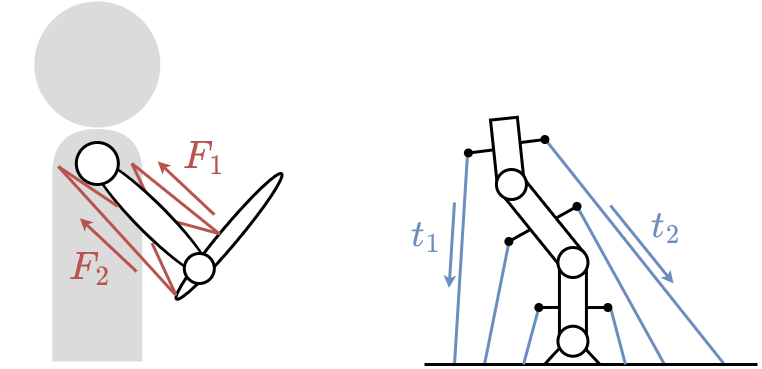
\includegraphics[width=\linewidth]{Chapters/imgs/muscle_mcdrs.png}
    \caption{An illustrative planar example of a human musculoskeletal model and a Multi-link cable-driven robot (MCDR). On the left human arm is modeled with two joints and six muscles, where each muscle can apply contraction forces $F_i$. On the right, a MCDR robot is modeled with 3 joints and 6 cables, which can apply tension forces $t_i$.  }
    \label{fig:muscle_mcdrs}
\end{wrapfigure}


 



One of the main differences comes from the actuator point of view. When it comes to MCDRs, the dynamics of the actuators is often neglected, considering them capable of instantaneously applying a range of $d$ tensile forces $\bm{t}\in\mathbb{R}^d$.
\begin{equation}
    \bm{t} \in [\bm{0},~\bm{t}_{max}]
\end{equation}
Additionally, this range is often considered constant and is not state dependent. For musculoskeleral models, on the other hand, the ranges of achievable muscle tension forces $\bm{F}$ are subject to many different biomechanical and biological factors, such as muscle length $\bm{l}$ and extension velocity $\dot{\bm{l}}$ as well the effects of fatigue and temperature.
Therefore the cables of the MCDRs can be seen as idealised muscles which tensile force capacity stays constant. 

Consequently, the physical ability metrics defined for the musculoskeleral models have the same formulation as the ones used to asses the performance of MCDRs.

\subsubsection{Wrench/Force polytope}
\label{ch:force_poly_human}
Task space force (or more generally wrench) capacity $\bm{f} \in \mathbb{R}^m$ is a well established metrics in biomechanics. It has been defined in two manners: a simplified formulation where the torques of $n$ human joints $\bm{\tau} \in \mathbb{R}^n$ are considered independent and limited (\ref{eq:human_torque_lim}) and in a more complete form where the human's joint torques $\bm{\tau}$ are generated by $d$ muscle tensile forces $\bm{F} \in \mathbb{R}^d$ which are limited in their respective ranges (\ref{eq:muslce_initial_range}).

Torque based polytopes \cite{rezzoug_application_2012,sasaki2011vertex} of achievable task space wrenches $\bm{f}$ have the same formulation as the force polytopes for robotic manipulators described in section \ref{ch:poly_force}. Therefore all the considerations for their evaluation are equivalent to those for robotic manipulators.  

However, real limits of human joint torques cannot be expressed as independent ranges (\ref{eq:human_torque_lim}) as they are generated by $d$ muscle tensile forces $\bm{F}$. The true limits of the joint torques $\bm{\tau}$ are polytope shaped as a consequence of the affine mapping of the muscle forces $\bm{F}$ to the joint space, though the moment arm matrix $N(\bm{q})=-L(\bm{q})^T$.
\begin{equation}
\mathcal{P}_\tau(\bm{q}) = \{\bm{\tau} \in \mathbb{R}^n ~|~\bm{F}\in [\bm{F}_{min}, \bm{F}_{max}], ~\bm{\tau}=N(\bm{q})\bm{F}\}
\label{eq:poly_torque_human}
\end{equation}

The relationship of the achievable task space wrenches $\bm{f}$ and the joint torques $\bm{\tau}$ is described through the dynamics equation 
\begin{equation}
\underbrace{M(\bm{q})\ddot{\bm{q}} + C(\bm{q},\dot{\bm{q}})\dot{\bm{q}} + \bm{g}(\bm{q})}_{\bm{\tau}_b(\bm{q},\dot{\bm{q}},\ddot{\bm{q}})} + J^T(\bm{q})\bm{f} = \bm{\tau} 
\end{equation}
where $\bm{\tau}_b(\bm{q},\dot{\bm{q}},\ddot{\bm{q}})$ is a state dependant joint torque bias vector including the influence of the gravity $\bm{g}(\bm{q})$ and human state $\{\dot{\bm{q}},\ddot{\bm{q}}\}$ and the desired acceleration $\ddot{\bm{q}}$. 

Finally the achievable set of task space wrenches $\bm{f}\in\mathbb{R}^m$ can then be expressed as a set of all the achievable wrenches $\bm{f}$ given the polytope $\mathcal{P}_\tau$ shaped limits of joint torques $\bm{\tau}$
\begin{equation}
    \mathcal{P}_f(\bm{q},\dot{\bm{q}},\ddot{\bm{q}}) = \left\{ \bm{f} \in \mathbb{R}^m ~|~ \bm{\tau}\in \mathcal{P}_\tau(\bm{q}), ~~ J^T(\bm{q})\bm{f} = \bm{\tau} -\bm{\tau}_b(\bm{q},\dot{\bm{q}},\ddot{\bm{q}}) \right\}
    \label{eq:human_force_poly_ver_poly_lim}
\end{equation}
Or in its implicit formulation
\begin{equation}
    \mathcal{P}_f(\bm{q},\dot{\bm{q}},\ddot{\bm{q}}) = \left\{ \bm{f} \in \mathbb{R}^m ~|~ \bm{F}\in\left[\bm{F}_{min}, \bm{F}_{max} \right], ~~ \!J^T(\bm{q})\bm{f} =\! N(\bm{q})\bm{F} -\bm{\tau}_b(\bm{q},\dot{\bm{q}},\ddot{\bm{q}}) \right\}
    \label{eq:human_force_poly}
\end{equation}

The final polytope formulation $\mathcal{P}_f$ has an implicit form composed of two affine mappings. First the limits of the muscle tension forces $\bm{F}\in \mathbb{R}^d$ are projected into the limits of the joint torques $\bm{\tau}\in \mathbb{R}^n$, then the polytope of the joint torques $\mathcal{P}_\tau$ is transformed to the task space wrenches $\bm{f}\in \mathbb{R}^m$ using the jacobian transpose matrix $J(\bm{q})^T$. As the musculoskeletal models often have large number of muscles $d$, the ending polytope $\mathcal{P}_f$ geometry is complex (having a large number of vertices and faces), both due to the number of muscles considered and the inherent complexity of the affine mapping. Therefore, this metric has been mostly used for static in-advance analysis of human postures \cite{hernandez_toward_2015}, due to its long execution times. 

However, Carmichael et al. \cite{carmichael_estimating_2013, carmichael2011Towards} have proposed a method capable of improving the time efficiency of the polytope resolution that has a potential to be used even in real-time applications. This method is based on Ray shooting method (RSM) that samples the polytope in a set of predefined direction in task space. By choosing the directions of interest in advance, the method is capable of approximating the polytope, however it does not give any guarantees on the approximation accuracy.

The achievable wrench polytope $\mathcal{P}_f$ formulation (\ref{eq:human_force_poly}) have been used for the analysis of the multi-link cable-driven robots (MCDRs) as well, for example in works by Sheng et al. \cite{sheng2020operational} or Muralidharan et al. \cite{Muralidharan2022}.

\subsubsection{Acceleration polytope}
\label{ch:human_aceleration_poly}

The task space acceleration polytope $\mathcal{P}_a$ describes the relationship between the limitation of the muscle tensile forces $\bm{F}\in \mathbb{R}^d$ and the set of achievable task space accelerations $\ddot{\bm{x}}\in\mathbb{R}^m$.

As in the case of the force polytope, the simplified approach to this metric is possible, where the human joint torque limits $\bm{\tau}\in\mathbb{R}^n$ are specified as independent ranges, resulting in the acceleration polytope formulation identical to the one for robotic manipulators, as introduced in section \ref{ch:accel_poly_robot}. 

However, human's joint torques $\bm{\tau}$ are not generated by a set of independent actuators, but with a set of $d$ contraction forces $\bm{F}$ produced by the muscle-tendon units $\bm{\tau}=N(\bm{q}) \bm{F}$. Therefore, real limits of achievable torques of human joints are polytope $\mathcal{P}_\tau$ shaped, as described by equation (\ref{eq:poly_torque_human}). 

The achievable acceleration polytope $\mathcal{P}_a$ formulation, respecting the muscle tension forces limits $\bm{F}$, can be derived from the human dynamics equation
\begin{equation}
M(\bm{q})\ddot{\bm{q}} + \underbrace{C(\bm{q},\dot{\bm{q}})\dot{\bm{q}} + \bm{g}(\bm{q}) + J^T(\bm{q})\bm{f}}_{\bm{\tau}_b(\bm{q},\dot{\bm{q}}, \bm{f})} = N(\bm{q}) \bm{F} 
\end{equation}
where $N(\bm{q})=-L(\bm{q})^T$ is the state dependant moment arm matrix. 
For any given human state $\{\bm{q},\dot{\bm{q}}, \bm{f}\}$, the effects of the human's motion, the gravity as well as the applied external wrenches, can be grouped in a constant torque vector $\bm{\tau}_b(\bm{q},\dot{\bm{q}},\bm{f})$. Then the actuator acceleration $\bm{q}$ can be expressed in relationship to the applied joint torque $\bm{\tau}$
\begin{equation}
    \ddot{\bm{q}} = M(\bm{q})^{-1}N(\bm{q})\bm{F} - M(\bm{q})^{-1}\bm{\tau}_b(\bm{q},\dot{\bm{q}}, \bm{f})
\end{equation}
Finally, the joint accelerations $\ddot{\bm{q}}$ can be transformed to the task space using the mapping (\ref{eq:js_to_cs_vaj_human:accel})
\begin{equation}
    \ddot{\bm{x}} = J(\bm{q})M(\bm{q})^{-1}N(\bm{q})\bm{F} - \underbrace{J(\bm{q})M(\bm{q})^{-1}\bm{\tau}_b(\bm{q},\dot{\bm{q}},\bm{f}) + \dot{J}(\bm{q}, \dot{\bm{q}})\dot{\bm{q}}}_{\bm{a}_b(\bm{q},\dot{\bm{q}},\bm{f})}
\end{equation}
where $\bm{a}_b(\bm{q},\dot{\bm{q}},\bm{f}) \in \mathbb{R}^m$ presents a constant bias vector for any human joint state $\{\bm{q},\dot{\bm{q}}\}$ and the genrated external wrench $\bm{f}$. The polytope $\mathcal{P}_a$ of achievable task space accelerations $\ddot{\bm{x}}$ can then be expressed as
\begin{equation}
\begin{split}
    \mathcal{P}_a(\bm{q},\dot{\bm{q}},\bm{f}) = \{ \ddot{\bm{x}} \in \mathbb{R}^m ~|~ \bm{F}&\in\left[\bm{F}_{min}, \bm{F}_{max} \right],\\ \ddot{\bm{x}} &= J(\bm{q})M(\bm{q})^{-1}N(\bm{q})\bm{F} - \bm{a}_b(\bm{q},\dot{\bm{q}},\bm{f}) \}
\end{split}
\label{eq:poly_acceleration_hum}
\end{equation}
The polytope $\mathcal{P}_a$ is formulated as a linear and affine projection of the muscles tension force $\bm{F}$ limits using the state dependant projection matrix $J(\bm{q})M(\bm{q})^{-1}N(\bm{q})$.  This polytope is much simpler to resolve than the force polytope $\mathcal{P}_f$ as it represents a projection of the $d$ dimensional limits of muscle tension forces $\bm{F}$ to the lower $m$ dimensional space of achievable task space accelerations $\ddot{\bm{x}}$.

Polytope $\mathcal{P}_a$ metrics have been used for musculoskeletal model analysis of highly dynamical movements such as football throwing \cite{khatib2009robotics} and golf swinging \cite{demircan2012muscle}. Additionally this metric has been used for the design analysis of the multi-link cable driven robots (MCDRs) as well \cite{sheng2020operational}.

\subsubsection{Velocity polytope}
\label{ch:human_vel_poly}
The simplest form of task space velocity capacity describes the relationship between the limited ranges (\ref{eq:human_js_vel_lim}) of human joint velocity $\dot{\bm{q}} \in \mathbb{R}^n$ and achievable task space velocities $\dot{\bm{x}} \in \mathbb{R}^m$, mapped through the jacobian matrix $J(\bm{q}) \in \mathbb{R}^{m\times n}$.
\begin{equation}
    \mathcal{P}_v(\bm{q}) = \left\{ \dot{\bm{x}} \in \mathbb{R}^m ~|~ \dot{\bm{q}}\in\left[\dot{\bm{q}}_{min}, \dot{\bm{q}}_{max} \right], ~~ \dot{\bm{x}} = J(\bm{q})\dot{\bm{q}} \right\}
\end{equation}
This formulation is essentially the same as the one for robotic manipulators described in velocity \ref{ch:vel_poly} and all the considerations discussed in that chapter are valid for this formulation as well.

However, taking in account only human's joint velocity $\dot{\bm{q}}$ limits in a form of independent ranges (\ref{eq:human_js_vel_lim}) does not take in consideration the limits of muscle extension velocity $\dot{\bm{l}}\in\mathbb{R}^d$. The true limits of human joint velocities are configuration dependent, as they are a consequence of the limits of muscle extension velocities $\dot{\bm{l}}$. The relationship between the joint and muscle extension velocities is given through the muscle jacobian matrix $L(\bm{q}) \in \mathbb{R}^{d\times n}$, forming polytope shaped limits
\begin{equation}
    \mathcal{P}_{\dot{q}}(\bm{q}) = \left\{ \dot{\bm{q}} \in \mathbb{R}^n ~|~ \dot{\bm{l}}\in\big[\dot{\bm{l}}_{min}, \dot{\bm{l}}_{max} \big], ~~ L(\bm{q})\dot{\bm{q}} = \dot{\bm{l}} \right\}
    \label{eq:human_poly_joint_vel}
\end{equation}
These polytope shaped limits can then be used to define the achievable task space velocity $\dot{\bm{x}}\in \mathbb{R}^m$ polytope which respects the limits of the muscle extension velocity $\dot{\bm{l}}$.
\begin{equation}
    \mathcal{P}_v(\bm{q}) = \left\{ \dot{\bm{x}} \in \mathbb{R}^m ~|~ \dot{\bm{q}}\in  \mathcal{P}_{\dot{q}}(\bm{q}), ~~ J(\bm{q})\dot{\bm{q}} = \dot{\bm{x}} \right\}
    \label{eq:velocity_polytope_human_ver_poly_lim}
\end{equation}
Or in its implicit form
\begin{equation}
    \mathcal{P}_v(\bm{q}) = \left\{ \dot{\bm{x}} \in \mathbb{R}^m ~|~ \dot{\bm{l}}\in\big[\dot{\bm{l}}_{min}, \dot{\bm{l}}_{max} \big], ~~ J(\bm{q})\dot{\bm{q}} = \dot{\bm{x}}, ~~ L(\bm{q})\dot{\bm{q}} = \dot{\bm{l}} \right\}
    \label{eq:velocity_polytope_human}
\end{equation}

This metric has an implicit formulation making its resolution relatively complex, requiring using multiple standard methods for polytope evaluation. It first requires finding the limits of joint velocities $\dot{\bm{q}} \in \mathbb{R}^n$ based on the limits of the muscle extension velocities $\dot{\bm{l}} \in \mathbb{R}^d$ and then projecting them to the task space velocities $\dot{\bm{x}} \in \mathbb{R}^m$. 

To the best of our knowledge, polytope $\mathcal{P}_v$ in its full implicit form (\ref{eq:velocity_polytope_human}), has not yet been used with musculoskeletal models. However, achievable velocity based physical ability metrics such as manipulability ellipsoids considering the joint velocity $\dot{\bm{q}}$ limits \cite{Chiu1988,Petric2019,Yang2017}, have been used in the human motion and ergonomics analysis. However, as these metrics neglect the the muscle extension velocity $\dot{\bm{l}}$ limits, polytope $\mathcal{P}_v$ could be used as their more complete alternative. 

The achievable velocity polytope $\mathcal{P}_v$, in the form (\ref{eq:velocity_polytope_human}), has been used for multi-link cable driven robots (MCDRs) analysis \cite{Muralidharan2022}.

\subsubsection{Stiffness polytope}
\label{ch:human_stiffness_poly}
Stiffness metrics for human musculoskeletal models are used to evaluate the limitations of the endpoint displacement $\Delta x \in \mathbb{R}^m$ given the known muscle stiffness matrix $K_m \in \mathbb{R}^{d\times d}$ and a limited range of task space wrenches $\bm{f} \in \mathbb{R}^m$. 

\begin{equation}
    \bm{f}\in\left[\bm{f}_{min}, \bm{f}_{max} \right]
    \label{eq:force_stiff_range_human}
\end{equation}

With a known muscle stiffness matrix $K_m$, that can be determined using the Hill's muscle model \cite{LATASH1993653}, the joint stiffness matrix $K_j\in \mathbb{R}^{n\times n}$ can be found using the muscle jacobian matrix $L(\bm{q}) \in \mathbb{R}^{d\times n}$
\begin{equation}
    K_j = L(\bm{q}) K_m L(\bm{q})^T 
\end{equation}
This joint space stiffness matrix $K_j$ can be used to find the robot state dependent task space stiffness $K_c  \in \mathbb{R}^{m\times m}$, through the jacobian matrix $J(\bm{q})\in\mathbb{R}^{m\times n}$  \cite{Salisbury1980,Ajoudani2018,Inouye2016}
\begin{equation}
     K_c(\bm{q})^{-1} = J(\bm{q}) K_j^{-1}J(\bm{q})^T
\end{equation}
Given the range of expected external wrenches (\ref{eq:force_stiff_range_human}), the polytope of maximal task space displacements $\Delta\bm{x}$ can then be expressed as
\begin{equation}
    \mathcal{P}_\Delta(\bm{q}) = \left\{ \Delta\bm{x} \in \mathbb{R}^m ~|~ \bm{f}\in\left[\bm{f}_{min}, \bm{f}_{max} \right], ~~ K_c(\bm{q})\Delta\bm{x} = \bm{f} \right\}
    \label{eq:stiffness_human_simple}
\end{equation}


However, this formulation considers that the external wrench $\bm{f}$ range (\ref{eq:force_stiff_range_human}) is inside the human wrench capacity. In order to make sure that the human's wrench capacity is not exceeded when calculating the maximal task space displacement polytope $\mathcal{P}_\Delta$ the external wrench range (\ref{eq:force_stiff_range_human}) needs to be intersected with the human's wrench polytope  $\mathcal{P}_f$ described in the section \ref{ch:force_poly_human}, the polytope $\mathcal{P}_\Delta$ of task space task space displacement $\Delta \bm{x}$ can then be expressed as
\begin{equation}
    \mathcal{P}_\Delta(\bm{q},\dot{\bm{q}},\ddot{\bm{q}}) = \left\{ \Delta\bm{x} \in \mathbb{R}^m ~|~ \bm{f}\in \left[\bm{f}_{min}, \bm{f}_{max} \right] \cap \mathcal{P}_f(\bm{q},\dot{\bm{q}},\ddot{\bm{q}}),  ~~ \! K_c(\bm{q})\Delta\bm{x}=\bm{f}\right\}
\end{equation}

If the maximal displacement polytope $\mathcal{P}_\Delta$ is calculated only in relationship to the human's wrench capacity $\mathcal{P}_f$, without specifying the expected range of external wrenches (\ref{eq:force_stiff_range_human}), this polytope can be expressed in an implicit form
\begin{equation}
\begin{split}
    \mathcal{P}_\Delta(\bm{q},\dot{\bm{q}},\ddot{\bm{q}}) =\! \{ \Delta\bm{x} \in \mathbb{R}^m ~|&\bm{F}\in\left[\bm{F}_{min}, \bm{F}_{max} \right]\!,\\ ~ &J^T(\bm{q})K_c(\bm{q})\Delta\bm{x}\!= N(\bm{q})\bm{F}\! -\! \bm{\tau}_b(\bm{q},\dot{\bm{q}},\ddot{\bm{q}}) \}\label{eq:stiffness_human_all}
\end{split}
\end{equation}
The stiffness polytope $\mathcal{P}_\Delta$ then represents the maximal task space displacement $\Delta \bm{x} \in \mathbb{R}^m$ that can be achieved given the human's muscle tensile forces $\bm{F} \in \mathbb{R}^d$ limits (\ref{eq:muslce_initial_range}), this polytope formulation is also called \textit{stiffness feasibility region} \cite{ajoudani2017choosing}.

The formulation of the polytope (\ref{eq:stiffness_human_simple}) has relatively low complexity, defined as a projection of the limits of the external task space wrenches $\bm{f} \in \mathbb{R}^m$ to the same dimensional task space displacements $\Delta \bm{x} \in \mathbb{R}^m$. However, the implicit polytope formulation (\ref{eq:stiffness_human_all}) is much more complex as the limits of muscle tension forces $\bm{F} \in \mathbb{R}^d$ first need to be projected to the limits of the joint torques $\bm{\tau} \in \mathbb{R}^n$ which in term determine the set of task space displacements $\Delta \bm{x} \in \mathbb{R}^m$. While the formulation  (\ref{eq:stiffness_human_simple}) can be resolved with standard polytope resolution algorithms, the formulation (\ref{eq:stiffness_human_all}) requires a combination of multiple methods, making it significantly more time consuming. 

These polytope based metrics however, to the best of our knowledge, have yet to be used with human musculoskeletal models and MCDRs. However, their potential has already been shown for human posture analysis \cite{Inouye2016} and MCDR design \cite{Ramadoss2021} applications, in their simplified ellipsoid forms.

\section{Polytope representation of collaboration abilities}
\label{ch:collab_metrics}

\begin{figure}[!h]
    \centering
    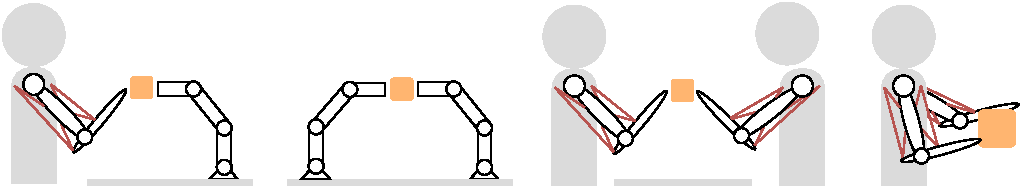
\includegraphics[width=\linewidth]{Chapters/imgs/collaboration.pdf}
    \caption{Illustrative examples of a common collaboration scenario composed of different actors (humans and robots), from left to right, human-robot, robot-robot, human-human and even two arms of a human subject can be seen as a collaboration of two musculoskeletal models.}
    \label{fig:collaboration_types}
\end{figure}

Physical ability metrics are an important tool for analysing how robots and humans comply with different requirements of tasks. In human-robot collaboration scenarios, these metrics can be used is to decide if the robot, or the human, is better suited to execute a certain task, by evaluating their different physical abilities (movement, forces, precision etc.) to the ones required by the task\cite{Edoardo2019Capability}. 

However, when it comes to the physical collaboration, where the task is executed jointly by the human and the robot physically interacting, expressing their common physical abilities is much more challenging. As their common physical ability is a combination of their individual abilities, to be able to calculate their common physical ability, they need to be expressed in a unified form.  

Many different physical abilities for humans and robots, can be represented in the polytope form, as described in section \ref{ch:poly_metrics}. Expressing their physical abilities in this unifying form enables using different efficient tools from the polytope algebra to combine their individual polytopes, such as Minkowski sums, intersections and convex-hulls.
Therefore, given their individual polytopes of different physical abilities and the physics of their physical interaction scenario, different polytope algebra operations can be leveraged to express their common physical ability in the polytope form as well.

One example of such characterisation has been developed by Jihong Lee, in his work \cite{lee2001velocity}, showing how polytopes can be used to describe the common velocity capacity of multi-arm collaborative robotic system, by intersecting their individual polytopes. However, this approach is yet to used for characterising the common capacity of the human-robot interaction, as well as to be extended to other physical abilities and other collaboration scenarios. 


Therefore, following sections describe the characterisation of different common physical abilities of the human-robot interaction, based on one classical example of human-robot collaboration scenario, where the two actors interact physically to manipulate an object that is rigidly fixed in the end-effector of the robot and in the hand of the human. First, section \ref{ch:which_metric_which} introduces the physical relationships describing this collaboration scenario, followed by the two sections, \ref{ch:force_collab} and \ref{ch:velocity_collab}, giving more specific examples of how these relationships are exploited to calculate the common force and velocity capacity of a physical human-robot collaboration leveraging the polytope algebra. 
Different versions of this scenario are shown on Figure \ref{fig:collaboration_types}, ranging from human-robot interaction to the interaction of the two arms of a human subject, that can be seen as two separate musculoskeletal models collaborating.

\todos{Even though the following sections are focusing on one collaboration scenario, similar approach can be used to characterising any other collaboration scenario as well.}

\subsection{Human-robot collaboration scenario}
\label{ch:which_metric_which}
\begin{wrapfigure}{r}{0.5\textwidth}
    \centering
    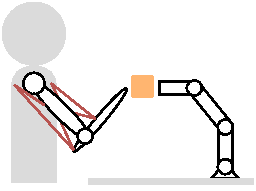
\includegraphics{Chapters/imgs/example_inter.pdf}
    \caption{A collaborative example scenario where a human and a robot interact over an object fixed rigidly in the end-effector of the robot and in the hand of the human.}
    \label{fig:table_inter}
\end{wrapfigure}

A classical human-robot physical interaction scenario is considered, where the human operator and the robot are physically interacting in order to manipulate an object which is rigidly fixed both in the robot's end-effector and the human's hand. A simplified view of this collaboration scenario is shown on Figure \ref{fig:table_inter}, while a more general view of this scenario, with different actors (humans and robots), is shown on Figure \ref{fig:collaboration_types}.

When it comes to commonly manipulating an object held by both human and the robot, the supposition of rigid contact with the object can be used to formulate the force equilibrium equation and the relative motion constraints \cite{Prattichizzo2016}. 

As they both apply forces on the object, the resulting force $\bm{f}$ the object will exert on the environment (if in contact with it) or transform into motion follows from the force equilibrium ( sum of all forces $\bm{f}_i$ is equal to zero ), and is equal to the sum of the applied forces by the robot $\bm{f}_r$ and the human $\bm{f}_h$. 
\begin{equation}
    \bm{f} = \bm{f}_r + \bm{f}_h, \qquad  m_o\ddot{\bm{x}} = \bm{f} 
\end{equation}
If the object is not in contact with the environment, the force $\bm{f}$ will generate object's acceleration $\ddot{\bm{x}}$  in space proportional to its mass $m_o$.

Furthermore, as the object is rigidly attached to both robot and the human, there is no relative movement possible between the object, human's hand and robot's end-effector. According to this condition, the movement of the object (velocity $\dot{\bm{x}}$, acceleration $\ddot{\bm{x}}$, jerk $\dddot{\bm{x}}$, etc.) is equivalent to the movement of both the human's hand $\{\dot{\bm{x}}_h,\ddot{\bm{x}}_h,\dddot{\bm{x}}_h\}$ and the robot's end-effector $\{\dot{\bm{x}}_r,\ddot{\bm{x}}_r,\dddot{\bm{x}}_r\}$.
\begin{equation}
    \dot{\bm{x}}_h=\dot{\bm{x}}_r=\dot{\bm{x}}, \qquad
    \ddot{\bm{x}}_h=\ddot{\bm{x}}_r=\ddot{\bm{x}}, \qquad
    \dddot{\bm{x}}_h=\dddot{\bm{x}}_r=\dddot{\bm{x}}
    \label{eq:kinematic_condition_contact}
\end{equation}

These two relationships, considering the rigid contact between the robot, human and the object, can be used to describe different physical abilities of the human-robot collaboration in the described scenario. Section \ref{ch:force_collab} describes exploiting this relationship to calculate the common force capacity while section \ref{ch:velocity_collab} described the calculation of their common velocity capacity.


% where each one of the forces is bounded in withing the polytope $\bm{f}_i \in \mathcal{P}_{fi}$. 
% \begin{equation}
%     \mathcal{P}_f = \{\bm{f}\in \mathbb{R}^m ~|~\bm{f} = \bm{f}_r + \bm{f}_h , \quad\bm{f}_r \in \mathcal{P}_{fr},~\bm{f}_h \in \mathcal{P}_{fh}\}
% \end{equation}
% Therefore their common wrench capacity can be expressed as a sum of their individual wrench capacities, corresponding to the Minkowski sum $\oplus$ in polytope algebra 
% \begin{equation}
%     \mathcal{P}_f = \mathcal{P}_{fr}\oplus \mathcal{P}_{fh}
% \end{equation}


% %the maximal velocity capacity of the object will be limited by the actor (human or robot) with the least velocity capacity. 

% On the other hand, in the proposed collaboration scenario, as both robot and the human are rigidly attached to the object, the velocity of the object $\dot{\bm{x}}$ is equal to the velocity of the human's hand $\dot{\bm{x}}_h$ and the robot's end-effector $\dot{\bm{x}}_r$ \cite{Prattichizzo2016}
% \begin{equation}
%     \dot{\bm{x}}_h=\dot{\bm{x}}_r=\dot{\bm{x}}
%     \label{eq:kinematic_condition_contact}
% \end{equation}
% as both of them have their own limited velocity capacity $\dot{\bm{x}}_h \in \mathcal{P}_{vh},\dot{\bm{x}}_r \in \mathcal{P}_{vr}$ the object velocity has to respect all of them
% \begin{equation}
%     \mathcal{P}_v = \{\dot{\bm{x}}\in \mathbb{R}^m ~|~ \dot{\bm{x}} \in \mathcal{P}_{vr},~\dot{\bm{x}} \in \mathcal{P}_{vh}\}
% \end{equation}
% Geometrically, this operation can be represented as an intersection of their velocity capacities, and the intersection $\cap$ operation can be calculated efficiently using polytope algebra. 
% \begin{equation}
%     \mathcal{P}_v =  \mathcal{P}_{vh} \cap \mathcal{P}_{vr}
% \end{equation}



% More generally, all the polytope formulations that require calculating the wrench/force capacity, for both robot's and human's, will be combined using Minkowski sum $\oplus$. Such metrics are human's and robot's wrench/force polytope and stiffness region polytope.

% More generally, all polytope metrics characterising robot's or human's movement capacity (velocity $\dot{\bm{x}}$, acceleration $\ddot{\bm{x}}$, etc.) will be subject to the same condition (\ref{eq:kinematic_condition_contact}) and will be combined using the intersection $\cap$ operation.




% The further discussed procedures for calculating joint physical ability polytopes are valid for the considered collaboration scenario (showed on Figure \ref{fig:table_inter} or more generally on Figure \ref{fig:collaboration_types}), however the same methodology can be used to any other collaboration scenario as well.

% \begin{table}
% \centering
% \begin{tabular}{|l|c | c| c| c|}
% \hline
% Polytope Metric & Equation & Dynamics & Collaboration operator \\
% \hline
%  \multicolumn{5}{c}{Robotic manipulators }  \\
% \hline
% Velocity  &  \ref{eq:poly_vel_rob}& No & $\cap$ \\
% Kinematic Acceleration  & \ref{eq:poly_accel_kin} & No & $\cap$ \\
% Kinematic Jerk  &  \ref{eq:poly_jerk_kin}& No &  $\cap$ \\
% Precision  & \ref{eq:poly_precision_rob} & No&  $\cap$ \\
% Force/Wrench  & \ref{eq:poly_force_rob} & Yes &$\oplus$ \\
% Acceleration  & \ref{eq:pol_accleration_rob} & Yes &   $\cap$ \\
% Stiffness feasibility  &  \ref{eq:pol_sfr_rob} & Yes& $\oplus$ \\
% \hline
%  \multicolumn{5}{c}{Human musculoskeletal models}  \\
% \hline
% Velocity  & \ref{eq:velocity_polytope_human} & No &  $\cap$ \\
% Force/Wrench & \ref{eq:human_force_poly} & Yes & $\oplus$ \\
% Acceleration  & \ref{eq:poly_acceleration_hum} & Yes &  $\cap$ \\
% Stiffness feasibility  & \ref{eq:stiffness_human_all}  & Yes&  $\oplus$ \\
% \hline
% \end{tabular}
% \caption{The list of common polytope based physical ability metrics alongside their polytope algebra operator for the example collaborative scenario (Figure \ref{fig:table_inter}), as well as the indication of their capacity to account for the dynamics effects.}
% \label{tab:table_comparisson_colloboration}
% \end{table}


\subsection{Force polytope}
\label{ch:force_collab}
\begin{figure}[!h]
    \centering
    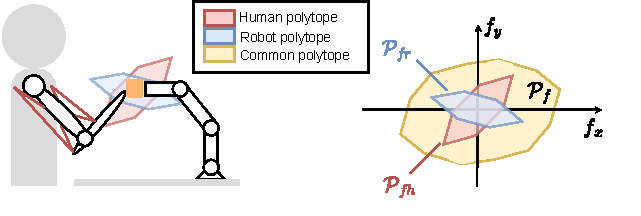
\includegraphics[width=0.7\linewidth]{Chapters/imgs/force_collab.pdf}
    \caption{A collaborative example scenario where a human and a robot interact over an object fixed rigidly in the end-effector of the robot and in the hand of the human. The force polytope of the human (red) and the robot (blue) as well as their collaborative polytope (orange) calculated as a Minkowski sum of their individual polytopes are shown on the right.}
    \label{fig:collaboration_force}
\end{figure}

When a human operator and a robot are physically interacting in order to manipulate an object, which is rigidly fixed both in the robot's end-effector and the human hand, the final force exerted on the object will be the sum of the forces of the human $\bm{f}_h$ and the force of the robot $\bm{f}_r$.
\begin{equation}
    \bm{f} = \bm{f}_h + \bm{f}_r
\end{equation}

Their individual force capacity can be expressed in a polytope form, for the human  $\mathcal{P}_{fh}$ and the robot  $\mathcal{P}_{fr}$ respectively. Finally, as their forces acting on the object are summed, their common force capacity on the object can be expressed as
\begin{equation}
    \mathcal{P}_f = \{\bm{f}\in \mathbb{R}^m ~|~\bm{f} = \bm{f}_r + \bm{f}_h , \quad\bm{f}_r \in \mathcal{P}_{fr},~\bm{f}_h \in \mathcal{P}_{fh}\}
\end{equation}
Therefore their common wrench capacity can be expressed as a sum of their individual wrench capacities, corresponding to the Minkowski sum $\oplus$ in polytope algebra 
\begin{equation}
    \mathcal{P}_f = \mathcal{P}_{fr}\oplus \mathcal{P}_{fh}
\end{equation}

A planar example of this collaboration scenario and the polytopes obtained is in shown on Figure \ref{fig:collaboration_force}. 

In more general case, if a collaboration is composed of $N$ actors rigidly holding an object, where their force capacity is expressed in a polytope form $\mathcal{P}_{fi}$, then their common force capacity can be calculated as the Minkowski sum of the $N$ polytopes.

\begin{equation}
    \mathcal{P}_f =  \mathcal{P}_{f1} \oplus \mathcal{P}_{f2} \oplus ~\ldots ~\oplus  \mathcal{P}_{fN}
\end{equation}

Furthermore, the polytope formulations that require calculating the wrench/force capacity, for both robot's and human's, will be combined using Minkowski sum $\oplus$. Such metrics are human's and robot's wrench/force polytope and stiffness region polytope, as shown in table \ref{tab:merged_table}.

\subsection{Velocity polytope}
\label{ch:velocity_collab}

\begin{figure}[!h]
    \centering
    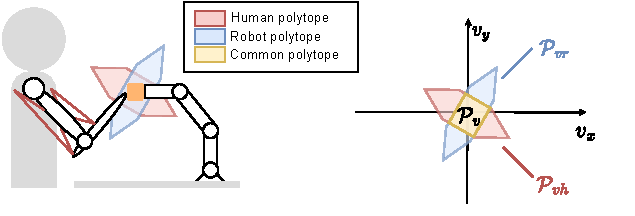
\includegraphics[width=0.7\linewidth]{Chapters/imgs/velocity_collab.pdf}
    \caption{A collaborative example scenario where a human and a robot interact over an object fixed rigidly in the end-effector of the robot and in the hand of the human. The velocity polytope of the human (red) and the robot (blue) as well as their collaborative polytope (orange) calculated as an intersection of their individual polytopes are shown on the right.}
    \label{fig:collaboration_vel}
\end{figure}

When a human operator and a robot are physically interacting in order to manipulate an object which is rigidly fixed both in the robot's end effector and the human hand, there is no relative movement of the object with respect to the human's hand and the robot's end effector
\begin{equation}
    \dot{\bm{x}}_h=\dot{\bm{x}}_r=\dot{\bm{x}},
\end{equation}

Once their individual velocity capacity is expressed in polytope form $\mathcal{P}_{vh}$ and $\mathcal{P}_{vr}$, their common velocity capacity $\mathcal{P}_v$ (the achievable velocities of the object) can then be calculated as 
\begin{equation}
    \mathcal{P}_v = \{\dot{\bm{x}}\in \mathbb{R}^m ~|~ \dot{\bm{x}} \in \mathcal{P}_{vr},~\dot{\bm{x}} \in \mathcal{P}_{vh}\}
\end{equation}
Geometrically, this operation can be represented as an intersection of their velocity capacities, and the intersection $\cap$ operation can be calculated efficiently using polytope algebra. 
\begin{equation}
    \mathcal{P}_v =  \mathcal{P}_{vh} \cap \mathcal{P}_{vr}
\end{equation}

A planar example of this collaboration scenario and the polytopes obtained is in shown on Figure \ref{fig:collaboration_vel}. 


% The maximal velocity the object can achieve in a certain direction $\bm{v}_{max}$ will be limited by the actor who has the lower maximal velocity in that direction. It can be found as the minimum value of the maximal velocity the human arm can achieve $\bm{v}_{h,max}$ and the robot's end-effector can achieve $\bm{v}_{r,max}$
% \begin{equation}
%     \bm{v}_{max}= \min \{\bm{v}_{h,max}, \bm{v}_{r,max}\}
% \end{equation}

In a more general case where there are $N$ actors (robots and humans) collaborating by rigidly holding the object, and where their velocity capacity is expressed in a polytope form $\mathcal{P}_{vi}$, the common velocity capacity can be calculated as their intersection
\begin{equation}
    \mathcal{P}_v =  \mathcal{P}_{v1} \cap \mathcal{P}_{v2} \cap ~~ \ldots ~~\cap \mathcal{P}_{vN}
\end{equation}

Furthermore, the polytope formulations characterising robot's or human's movement capacity (velocity $\dot{\bm{x}}$, acceleration $\ddot{\bm{x}}$, etc.) will be subject to the same condition (\ref{eq:kinematic_condition_contact}) and will be combined using the intersection $\cap$ operation, as shown in table \ref{tab:merged_table}.

\section{Conclusion and synthesis}
\label{ch:collab_metrics_overview}

This chapter brings an overview of different ways of characterising physical abilities for humans and robots, with the aim to find a unified view of their abilities and provide a base for characterising their common physical abilities. Even though many different metrics have been developed for human and robot physical ability characterisation, they are often very different in scope, accuracy, physical interpretation and in many cases specific to only robots or only humans. The focus of this chapter, as well as this thesis, is therefore placed on polytope based representations of physical abilities as they are arguably the most complete and the most accurate characterisations for both robots and humans, based on their musculoskeletal models.

An overview of the common polytope based representations of humans' and robots' physical abilities is then provided in section \ref{ch:poly_metrics}, in the attempt to present a systematic view on their formulations. In this overview, different physical abilities of humans (based on musculoskeletal models) and robots are characterised by finding the relationships between their actuation limits and the achievable sets of different task-related variables. As these relationships are usually described through robot's and human's highly nonlinear dynamics and kinematics relationships, in order to obtain the polytope-shaped representations, the dynamics and kinematics equations are linearised around a specific state, yielding linear and affine transformations of the actuator limits to the achievable sets of desired task space variables.

Common polytope formulations, described in section \ref{ch:robot_metrics} for robots and in section \ref{ch:human_metrics} for humans, involve different linearised dynamics and kinematics equations, as well as different actuation limits. However, they can be represented using a generic formulation
\begin{equation}
    \mathcal{P}_x = \{\bm{x}\in\mathbb{R}^m ~|~ A\bm{x}=B\bm{y} + \bm{b}, ~ \bm{y}\in\mathcal{P}_y\}
    \label{eq:generic_polyt_view}
\end{equation}
where the polytope $\mathcal{P}_x$ represents the achievable set of the task space variable $\bm{x}\in\mathbb{R}^m$, $\bm{y}\in\mathbb{R}^k$ is the input (actuator) variable limited within input set (actuator limits) $\mathcal{P}_y$. The input set $\mathcal{P}_y$ is often defined in the form of intervals of different input (actuator) variables, however in general case it can have a polytope shape as well. The linearised dynamics and kinematics equations can be represented, in a generic case, using the equation $A\bm{x}\!=\!B\bm{y}\!+\!\bm{b}$, where the matrix $A\in\mathbb{R}^{k\times m}$ is a linear transformation matrix from the $m$ dimensional output (task) space to the $k$ dimensional intermediate space, the matrix $B\in\mathbb{R}^{k\times d}$ is a transformation matrix from the $n$ dimensional input space to the intermediate space and the $\bm{b}\in\mathbb{R}^k$ is a bias vector expressed in the intermediate space. Furthermore, the dimensions of output (task) space $m$ is lower than the intermediate space dimension $k\!\geq\! m$ , which is in term lower than the input (actuator) space dimension $n\!\geq\! k\!\geq\! m$. This condition comes from the fact that when characterising the physical abilities, the polytopes map higher dimensional input space (ex. joint space or muscle force space) to the lower dimensional output space (ex. Cartesian space).

\begin{table}[!b]
\scalefont{0.9}
\centering
\begin{tabular}{|l|c|c|c|c|c|c|c|c|c|}
\hline
Polytope capacity & Eqn. & $\bm{x}$ & $A$ & $B$ & $\bm{y}$ & Input set $\mathcal{P}_y$ & $\bm{b}$ & Cond. & Collab. \\
\hline
\multicolumn{10}{c}{Robotic manipulators} \\
\hline
Velocity & \ref{eq:poly_vel_rob}& $\dot{\bm{x}}$ & $I_{m\times m}$ & $J$ & $\dot{\bm{q}}$& $[\dot{\bm{q}}_{min},\dot{\bm{q}}_{max}]$ & - & Kin & $\cap$ \\
Kin. Acceleration & \ref{eq:poly_accel_kin} & $\ddot{\bm{x}}$ & $I_{m\times m}$ & $J$ & $\ddot{\bm{q}}$ & $[\ddot{\bm{q}}_{min},\ddot{\bm{q}}_{max}]$ & $\bm{a}_b$ & Kin & $\cap$ \\
Kin. Jerk &\ref{eq:poly_jerk_kin} & $\dddot{\bm{x}}$ & $I_{m\times m}$ & $J$ & $\dddot{\bm{q}}$& $[\dddot{\bm{q}}_{min},\dddot{\bm{q}}_{max}]$ & $\bm{j}_b$ & Kin & $\cap$ \\
Precision & \ref{eq:poly_precision_rob} & $\delta\dot{\bm{x}}$ & $I_{m\times m}$ & $J$ & $\delta\bm{q}$ &$[\delta{\bm{q}}_{min},\delta{\bm{q}}_{max}]$ & - & Kin & $\cap$ \\
Force/Wrench & \ref{eq:poly_force_rob} & $\bm{f}$ & $J^T$ & $I_{n\times n}$ & $\bm{\tau}$ &$[\bm{\tau}_{min},\bm{\tau}_{max}]$ & -$\bm{\tau}_b$ & Dyn & $\oplus$ \\
Acceleration & \ref{eq:pol_accleration_rob} & $\ddot{\bm{x}}$ & $I_{m\times m}$ & $JM^{-1}$ & $\bm{\tau}$ &$[\bm{\tau}_{min},\bm{\tau}_{max}]$ & -$\bm{a}_b$ & Dyn & $\cap$ \\
Stiffness & \ref{eq:pol_sfr_rob}& $\Delta\bm{x}$ & $J^TK_c$ & $I_{n\times n}$ & $\bm{\tau}$ &$[\bm{\tau}_{min},\bm{\tau}_{max}]$ & -$\bm{\tau}_b$ & Dyn & $\oplus$ \\
\hline
\multicolumn{10}{c}{Human musculoskeletal models} \\
\hline
Velocity &\ref{eq:velocity_polytope_human} & $\dot{\bm{x}}$ & $I_{m\times m}$ & $J$ & $\dot{\bm{q}}$ & $\mathcal{P}{\dot{\bm{q}}}$ & - & Kin & $\cap$ \\
Force/Wrench & \ref{eq:human_force_poly} & $\bm{f}$ & $J^T$ & $N$ & $\bm{F}$ & $[\bm{F}_{min},\bm{F}_{max}]$ & -$\bm{\tau}_b$ & Dyn & $\oplus$ \\
Acceleration & \ref{eq:poly_acceleration_hum} & $\ddot{\bm{x}}$ & $I_{m\times m}$ & $JM^{-1}N$ & $\bm{F}$ & $[\bm{F}_{min},\bm{F}_{max}]$ & -$\bm{a}_b$ & Dyn & $\cap$ \\
Stiffness & \ref{eq:stiffness_human_all} &$\Delta\bm{x}$ & $J^TK_c$ & $N$ & $\bm{F}$ & $[\bm{F}_{min},\bm{F}_{max}]$ & -$\bm{\tau}_b$ & Dyn & $\oplus$ \\
\hline
\end{tabular}
\caption{The list of common polytope formulations for characterising physical abilities of robots and humans introduced in section \ref{ch:poly_metrics}. The table shows the correspondence of the common formulations to the generic formulation described by the equation (\ref{eq:generic_polyt_view}). The table further specifies if the polytope formulations is specified in kinematic or dynamic conditions. Finally, the table shows the necessary polytope algebra operator in order to characterise the common abilities in the collaboration scenario described in section \ref{ch:which_metric_which}.}
\label{tab:merged_table}
\end{table}

Table \ref{tab:merged_table} brings a list of the polytope formulations for robots and humans, introduced in section \ref{ch:poly_metrics}, in a condensed view. The table brings shows how different polytope formulations correspond with the generic polytope formulation (\ref{eq:generic_polyt_view}), in terms of system matrices $A,B$, input, output and bias vectors $\bm{x},\bm{y},\bm{b}$ and the input limits $\mathcal{P}_y$.

Polytopes, apart from being able to accurately represent both human's and robot's physical abilities, enable combining their individual polytopes for characterising the common physical abilities when interacting physically to execute different task. Given the physical ability of interest and the physics of the human-robot physical interaction scenario, different polytope algebra tools, such as Minkowski sum or intersection, can be used to express the common physical ability of their interaction in the polytope form as well.


Section \ref{ch:collab_metrics}, demonstrates the use of different polytope algebra operations to characterise force and movement capacity of the human-robot collaboration in one classical collaboration scenario, where the human and the robot jointly manipulate an object. In the context of the same scenario, table \ref{tab:merged_table} shows the polytope algebra operators (Minkowski sum $\oplus$ and intersection $\cap$) used to combine their individual polytopes to characterise their different physical abilities as one system.


In summary, polytopes enable accurate representation of human's and robot's physical abilities, as well as characterising their common physical abilities when collaborating physically to execute a task. In that way, this representation provides tools to create more advanced collaboration scenarios. 
Accurate representation of robot's physical abilities enables exploiting its abilities fully when designing its tasks, creating the adapted robot control strategies or planning for its trajectories. On the other hand, accurate representation of human's abilities enables assessing the task ergonomics and making sure that human's capacity is never surpassed. Additionally, it enables creating more human-centered robot behaviours, where the robot adapts its assistance level to the lacking physical abilities of the human operator. 
Finally, a unified representation of their individual and common physical abilities might enable new task scheduling techniques capable of assessing if different tasks are more suitable for robots, human operators or are they more suitable for their collaboration. 

However, polytope formulations, as introduced in section \ref{ch:poly_metrics}, need to be transformed to more standard representations in order to  be used in practical implementations. The two most common ways to represent a polytope are as a set of vertices, or as a set of inequality constraints corresponding to its faces. Depending on the polytope formulation structure different transformation strategies, to the one of these forms, need to be employed, where the computational efficiency of the transformation operation can vary significantly with respect to the formulation complexity. Therefore following chapter focuses on providing a generic view on different formulation families present when characterising physical abilities of humans and robots, with the aim to specify different polytope transformation strategies applicable to each of the families as well as to discuss their computational complexity.


% \pagebreak

% \begin{landscape}
% \centering
% \begin{table}[!h]
% \centering
% \begin{tabular}{|l|c|c|c|c|c|c|c|c|c|}
% \hline
% Polytope capacity & Equation & $\bm{x}$ & $A$ & $B$ & $\bm{y}$ & Input set $\mathcal{I}$ & $\bm{b}$ & Conditions & Collaboration \\
% \hline
% \multicolumn{10}{c}{Robotic manipulators} \\
% \hline
% Velocity & \ref{eq:poly_vel_rob}& $\dot{\bm{x}}$ & - & $J$ & $\dot{\bm{q}}$& $[\dot{\bm{q}}_{min},\dot{\bm{q}}_{max}]$ & - & Kin & $\cap$ \\
% Kin. Acceleration & \ref{eq:poly_accel_kin} & $\ddot{\bm{x}}$ & - & $J$ & $\ddot{\bm{q}}$ & $[\ddot{\bm{q}}_{min},\ddot{\bm{q}}_{max}]$ & $\bm{a}_b$ & Kin & $\cap$ \\
% Kin. Jerk &\ref{eq:poly_jerk_kin} & $\dddot{\bm{x}}$ & - & $J$ & $\dddot{\bm{q}}$& $[\dddot{\bm{q}}_{min},\dddot{\bm{q}}_{max}]$ & $\bm{j}_b$ & Kin & $\cap$ \\
% Precision & \ref{eq:poly_precision_rob} & $\delta\dot{\bm{x}}$ & - & $J$ & $\delta\bm{q}$ &$[\delta{\bm{q}}_{min},\delta{\bm{q}}_{max}]$ & - & Kin & $\cap$ \\
% Force/Wrench & \ref{eq:poly_force_rob} & $\bm{f}$ & $J^T$ & - & $\bm{\tau}$ &$[\bm{\tau}_{min},\bm{\tau}_{max}]$ & -$\bm{\tau}_b$ & Dyn & $\oplus$ \\
% Acceleration & \ref{eq:pol_accleration_rob} & $\ddot{\bm{x}}$ & - & $JM^{-1}$ & $\bm{\tau}$ &$[\bm{\tau}_{min},\bm{\tau}_{max}]$ & -$\bm{a}_b$ & Dyn & $\cap$ \\
% Stiffness & \ref{eq:pol_sfr_rob}& $\Delta\bm{x}$ & $J^T$ & - & $\bm{\tau}$ &$[\bm{\tau}_{min},\bm{\tau}_{max}]$ & -$\bm{\tau}_b$ & Dyn & $\oplus$ \\
% \hline
% \multicolumn{10}{c}{Human musculoskeletal models} \\
% \hline
% Velocity &\ref{eq:velocity_polytope_human} & $\dot{\bm{x}}$ & - & $J$ & $\dot{\bm{q}}$ & $\mathcal{P}{\dot{\bm{q}}}$ & - & Kin & $\cap$ \\
% Force/Wrench & \ref{eq:human_force_poly} & $\bm{f}$ & $J^T$ & $N$ & $\bm{F}$ & $[\bm{F}_{min},\bm{F}_{max}]$ & -$\bm{\tau}_b$ & Dyn & $\oplus$ \\
% Acceleration & \ref{eq:poly_acceleration_hum} & $\ddot{\bm{x}}$ & - & $JM^{-1}N$ & $\bm{F}$ & $[\bm{F}_{min},\bm{F}_{max}]$ & -$\bm{a}_b$ & Dyn & $\cap$ \\
% Stiffness & \ref{eq:stiffness_human_all} &$\Delta\bm{x}$ & $J^TK_c$ & $N$ & $\bm{F}$ & $[\bm{F}_{min},\bm{F}_{max}]$ & -$\bm{\tau}_b$ & Dyn & $\oplus$ \\
% \hline
% \end{tabular}
% \caption{Comparison of Polytope-based Physical Ability Metrics}
% \label{tab:merged_table}
% \end{table}
% \end{landscape}